\documentclass[12pt, a4paper]{scrreprt}

\renewcommand*\familydefault{\sfdefault} 
%\usepackage[T1]{fontenc}

\usepackage[english]{babel}
%\usepackage{cite}
\usepackage[utf8]{inputenc}
%\usepackage[onehalfspacing]{setspace}
\usepackage{geometry, textcomp}
\newgeometry{right=2cm,left=4cm, top=2.5cm, bottom=2.3cm, footnotesep=0.5cm}
%\usepackage[acronym]{glossaries}

\usepackage[printonlyused]{acronym}  % Abkürzungsverzeichnis [nur verwendete Abkürzugen]

%\glsenablehyper

%\makeglossaries

\usepackage{savesym}
\usepackage{amsmath,amssymb,amstext}
%\usepackage{graphics}
\savesymbol{iint}
\usepackage{txfonts}

\restoresymbol{TXF}{iint}
\usepackage[automark,headsepline,ilines,komastyle]{scrpage2}
\usepackage{blindtext}
\usepackage[euler]{textgreek}
\setlength{\parindent}{0pt}
\setlength{\headheight}{1.5\baselineskip}
\renewcommand{\baselinestretch}{1.5}

\pagestyle{scrheadings}
\clearscrheadfoot
\ihead[]{}
\chead[]{}
\ohead[]{\headmark \hfill \thepage}
\ifoot[]{}
\cfoot[]{}
\ofoot[]{}

\setheadsepline[\textwidth]{1pt}
\usepackage{tabularx}
\usepackage{colortbl}
\usepackage{multirow}
\usepackage{hhline}
\usepackage{array}
\usepackage{tocloft}
\usepackage[hidelinks]{hyperref}
\tocloftpagestyle{scrheadings}
\renewcommand{\chapterpagestyle}{scrheadings}
\usepackage[font=footnotesize]{caption}

\usepackage{tikz}
\usepackage{rotating} 

\newenvironment{packed_item}
	{\begin{itemize}
			\setlength{\itemsep}{0pt}
			\setlength{\topsep}{0pt}
			\setlength{\parsep}{0pt}
			\setlength{\parskip}{0pt}}
		{\end{itemize}}
	
\usepackage[style=authoryear, natbib=true, backend=biber]{biblatex}

\renewcommand{\nameyeardelim}{ }
\usepackage[babel,german=guillemets]{csquotes}

\makeatletter

\newrobustcmd*{\parentexttrack}[1]{%
	\begingroup
	\blx@blxinit
	\blx@setsfcodes
	\blx@bibopenparen#1\blx@bibcloseparen
	\endgroup}

\AtEveryCite{%
	\let\parentext=\parentexttrack%
	\let\bibopenparen=\bibopenbracket%
	\let\bibcloseparen=\bibclosebracket}

\makeatother

\usepackage{pstricks}
\usepackage{pstricks-add}

\bibliography{Lit.bib}

\usepackage[final]{pdfpages}

\begin{document}
		\begin{titlepage}
			\begin{center}
			%\setlength{\headheight}{1.5\baselineskip}
			\renewcommand{\baselinestretch}{1.5}
					\textbf{\large FOM - Hochschule für Oekonomie \& Management \\
						Hamburg \\
						\ \\
						Master-Studiengang Big Data \& Business Analytics \\
						3. Semester \\
						\ \\
						Development of a system to control and monitor blood pressure \ \\
						measurements to prevent cardiovascular disease \ \\
						\ \\
						}
						
					\textrm{
						\ \\
						Betreuer: Prof. Dr. Kai Brüssau \\
						\ \\
						Autor: Jacqueline Franßen \\
						\ \\
						Matrikel-Nr: 496804 \\
						\ \\
						3. Fachsemester \\
						\ \\
						Hamburg, den 29.02.2020 \\
						}
			\end{center}
		\end{titlepage}

%\includepdf{Image/Deckblatt.pdf}

			\setcounter{tocdepth}{3}
			\setcounter{secnumdepth}{3}		
			\pagenumbering{Roman}
			\thispagestyle{empty}
			\pdfbookmark{\contentsname}{toc}\tableofcontents
			\newpage
			\listoffigures
			\listoftables

			\pagenumbering{arabic}
			\thispagestyle{empty}
\chapter{Abstract}\label{abstract}

This scientific article focusses on the development of a neural network to detect tumors and to prevent skin cancer from recurring.
The main purpose of this scientific article is to develop a model to be able to detect a specific type of skin cancer automatically.
What is more, the mobile app should connect both patients and healthcare practitioners by digitalizing all measured data and saving them centrally on a secured database. 
The first business case is that patients are frequently reminded of going to a control appointment. 
Second, by using their smartphone's hardware, especially the camera can be used to take a photo of potential skin cancers. 

\chapter{Introduction}\label{introduction}

\section{Problem statement}

One of the most popular disease in our modern society is cancer. Many people die because of the consequences of tumors, evolving in their bodies and capturing nearly all of their good, healthy cells. The cause of tumors is the mutation of cells into 'bad' cells which clone themselves uncontrolled and irregularly. This makes it very hard to diagnose and prevent new tumors. Sometimes, even experts cannot diagnose precisely, e.g. in case of malignant tumors which are not delimited in the \ac{mri} pictures but tend to proliferate in an unknown degree. Another problem is the point of time the diagnosis is made. Since many people who do not suffer from any chronic disease tend to go to the doctor infrequently, the tumor is be detected too late. What is more, most biopsies take up to multiple days which is a long time.

\section{Aim and scope of this work}

Given the above explained problems, the goals are to improve diagnostic and treatment of tumor patients by developing a model which predicts tumor metastasis and recurrence. Moreover, the system shall help doctors to quickly identify a patient whose cells are mutating so that he can intervene and treat the patient at the right time. Furthermore, the information process shall be improved by setting up a mobile and web application which keeps the patients up to date and serves as a communication base for healthcare providers.

%describe aim
The first aim of this scientific work is to develop a solution ...
%describe scope
What is important, the developed model is only a reference model....

\chapter{Fundamentals}\label{fundamentals}

\section{Related Work}

Deep learning methods use multiple layers of nonlinear processing units for feature extraction and transformation and to find deep relationships between complex variations under supervised and unsupervised procedures.

\subsection{\ac{iarc}}

The \ac{iarc} is a association with the aim to raise the development within cancer treatment and research. It was formed by the \ac{who} and has its main location in France. Besides, it provides a large library of cancerogens for users.

\footnote{\cite{iarc_world_cancer_report}}

\subsection{Ultrawideband, Stable Normal and Cancer Skin Tissue Phantoms for Millimeter-Wave Skin Cancer Imaging}

\footnote{\cite{8344452}}

\subsection{Identification of 12 cancer types through genome deep learning}

Sun et al. constructed '14 models including 12 specific models, a total-specific model and a mixture model for cancer risk identification using a \ac{dnn} within a TensorFlow23 framework. We used an exponential decay method to optimize the learning rate, L2 regularization24 to minimize overfitting, and a sliding average model to increase the robustness of the model. For each specific model meant to identify a certain type of cancer, the detection accuracy, sensitivity and specificity are more than 97\%, 98\% and 97\%, respectively. The mixture model, which is able to distinguish all 12 types of cancer, exhibited comparable performance. The total-specific and mixture models also demonstrated comparable performance. Using our model, cancerous tissue can be identified more conveniently and timely, thus providing an opportunity for earlier treatment. This approach to genome deep learning offers a new direction for disease diagnosis while providing a new method to predict traits based on genomic information.'\footnote{\cite{sun_identification}}

Besides, Sun et al. mention multiple deep learning methods, such as 'Alpha Go' and object recognition which are used to recognize the locations of splice site promoters and enhancers in genetics. Furthermore, these are able to predict proteins secondary structure and functions.

Another advantage of using AI algorithms in cancer research is that they could achieve higher tumor-level sensitivity than pathologists. To give an example, today it is possible to automatically detect cerebral microbleeds from \ac{mr} images which were identified by 3D \ac{cnn}s.

\subsection{\ac{ham10000}}
Dermatoscopy TBD 
\footnote{\cite{ham10000}}

%\subsection{canscreen}
\subsection{\ac{canscreen5}}

The \ac{iarc} provides many projects based on different data sources. One large project is the \ac{canscreen5}\footnote{\cite{iarc_canscreen5_project}} which collects all information on several cancer screening programmes across the globe. Thereby, the main goals are quality improvement and effective programme evaluation of cancer therapies. There are three types of cancer (breast, cervical and colorectal cancer) which are examined precisely. Besides, an overall graphic explains the distribution of cancer types across the worldwide population. Furthermore, the \ac{canscreen5} project provides analysis tools to be able to see the distribution of for example breast cancer in european countries.  

\section{Different types of skin tumors}

'The skin is made of a variety of cells, many of which are in constant motion. Round basal cells below the surface flatten as they rise to replace dead, flaking squamous cells on the surface. Melanocytes tan the skin in the sunlight, and Merkel cells give skin its ability to sense touch. When these cells become damaged, they may develop into skin cancer.' \footnote{\cite{skin_cancer_types}} 

\begin{table}[h!]
\begin{center}
 \begin{tabular}{|| c | c | c ||} 
 \hline
Tumor Name & Description & Benign/Malignant \\ [0.5ex] 
\hline\hline
Basal Cell Carcinoma & tbd & tbd \\
\hline
Recurrent Basal Cell Carcinoma & tbd & tbd \\
 \hline
 Squamous Cell Carcinoma & tbd & tbd \\
 \hline
Melanoma & tbd & tbd \\
 \hline
 Karposi sarcoma (Rare Skin cancer) & tbd & tbd \\
 \hline
  Actinic keradosis (Rare Skin cancer) & tbd & tbd \\
\hline
Lymphoma of the skin (Rare Skin cancer) & tbd & tbd \\
\hline
 Keratoacanthoma (Rare Skin cancer) & tbd & tbd \\
\hline
 Merkel Cell Carcinoma & tbd & tbd \\
 \hline
\end{tabular}
\caption{Different types of skin cancers} \label{table}         

\end{center}
\end{table}




As described by \ac{ndr} \footnote{\cite{ndr_lymphom}}, malignant skin lymphoma are caused by our immunesystem cells (also knows as lymphocytes). In such case, the lymphocytes are collected beneath the skin, grow uncontrolled and cause lymphomes. The reason for the mutation and why these cells cause skin lymphomes is unknown.

\subsection{Current diagnosis and therapy methods}

When assuming skin lymphoma, doctors often examine the patient's blood or use X-ray and ultrasound to detect all tumor cells. 
After recognizing all malignant cells, there are several therapy methods, such as cortisone ointment, phototherapy, extracorporeal photopheresis, X-rays, antibody therapy, chemotherapy and symptomatic therapy.

Given these numerous therapy methods, it is very important to diagnose the 'right' disease. Often, lymphoma tend to mutate and hide themselves as psoriasis and are treated like them for many years. But suddenly, the doctor notices that it is not a usual psoriasis and the lymphoma can immediately lead to the patient's death. For that reason, the diagnosis process should be repeated like a cycle and should include all different data sources (e.g. not only image recognition but also blood analysis) \footnote{\cite{ndr_lymphom}}. 

\subsection{Stages of skin cancer}

When diagnosing tumors, a often used scale is the \ac{tnm} grading which describes the current stage of the tumor. 
Tumor (t) describes the tumor's size, location and how deep it has grown into the skin. Node (n) indicates whether or not the cancer cells have spread to nearby lymph nodes or the channels connecting the lymph nodes. Metastasis (m) refers to whether the cancer cells have spread to distant organs.
The table \ref{table_tnm} shows all possible classifications of tumors, according to the German Cancer Organization\footnote{\cite{dkgs_tumor_classification}}. These can be identified internationally and are used when diagnosing tumors to give further information about the treatment. For instance, tumors with a lower stage like 0 do not need a high regulated therapy or medication than tumors with a higher stage like 4.

\begin{table}[h!]
\begin{center}
\begin{tabularx}{\textwidth}{|XX|}
  \textbf{Stage} & \textbf{Tumor development} \\
\hline
0 & 'Carcinoma in situ', tumor is only present in the epidermis (upper layer of the skin) and has not spread deeper to the dermis \\
1 & cancer is less than 2 centimeters, about 4-5 of an inch across, has not spread to nearby lymph nodes or organs, and has one or fewer high-risk features  \\
2 & cancer is larger than 2 centimeters across, and has not spread to nearby organs or lymph nodes, or a tumor of any size with 2 or more high-risk features \\
3 & cancer has spread into facial bones or 1 nearby lymph node, but not to other organs  \\
4 & cancer can be any size and has spread (metastasized) to 1 or more lymph nodes which are larger than 3 cm and may have spread to bones or other organs in the body \\
\end{tabularx}
\caption{Tumor Classification according to German Cancer Organization} \label{table_tnm}         
\end{center}
\end{table}

According the the detected stage, the therapy is personalized. For instance, if tumors are in stage 1, a more simple treatment is administered whereas tumors in stage 4 have to be treated using more aggressive therapies, such as chemotherapies.   

Besides, there are additional criteria which can determine a higher risk for recurrence or spreading. These are for example a thickness greater than 2mm, invasion into the lower dermis or tiny nerves in the skin or a location on the ear or on a hair-bearing lip\footnote{\cite{skin_cancer_types}}.

\section{Current algorithms, solutions to recognize skin tumors and to predict metastasis}

\section{Overview: Apps to predict metastasis}

There already exist some applications to predict certain types of cancer worldwide, such as \footnote{\cite{iarc_predict_cancer_worldwide}}. These solutions provide several information about the tumors by showing them within many different types of charts. They do not specify on a certain patient (which would also cause problems with data privacy and protection) but explain them in general.  

\subsection{Yuma App}
a mobile app to protect against sunburning

\footnote{\cite{vijini_gen_alg}}


\chapter{Image Recognition and App Development}
Here all used algorithms and patterns shall be explained

\section{Image Recognition}
\section{Hybride App Development}

\subsection{Native Development with NativeScript} 

There are several ways to create a mobile application, like for example with Android Studio or iOS. But the challenge is to develop a hybrid solution for both systems at the same time.
To face that challenge, Nativescript has been established as an open-source project from Telerik in the last years \footnote{\cite{nativescript}}. 

The free and open source technology enables developers to easily build cross-platform native apps with either Javascript, Nativescript or by using Angular \footnote{\cite{nativescript}}. 
Regarding its design philosophy, Nativescript was designed to be approachable to developers from various backgrounds \footnote{\cite{nativescript}}. Moreover, it was designed to be both performant and giving access to native APIs, such as Android or iOS.

Figure \ref{nsarchitecture} gives an impression of the general architecture of Nativescript applications. When developing such applications, one of the given frameworks can be used (e.g. 'N Core' which is basic Javascript, Angular or Vue). Additionally, several Nativescript plugins can be selected. Below the 'NativeScript Core Modules', there are located the 'NativeScript Runtimes' which have direct access to the Native system. By running several commands on the NativeScript \ac{cli}, the developed Nativescript application can be executed on any physically connected device as well as on the installed emulator or in the cloud. 

\begin{figure}[h!]
	\centering
	\includegraphics[width=1\textwidth]{images/ns-architecture.png}
	\caption{The architecture of NativeScript Applications, adopted from Nativescript}
	\label{nsarchitecture}
\end{figure}

NativeScript applications can also be developed, built and run on the 'NativeScript Playground' \footnote{\cite{nsplayground}} which enables independent development. Moreover, NativeScript Playground is easier to handle because the application is executed in the Cloud. Generally, by offering a user-friendly surface, NativeScript Playground is appropriate for beginners who start developing native mobile applications.

\subsubsection{NativeScript Application Logic}

\begin{figure}[h!]
	\centering
	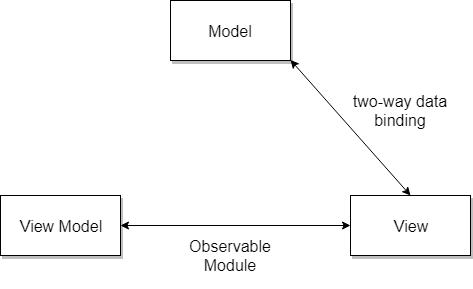
\includegraphics[width=1\textwidth]{images/mvvm_ns.png}
	\caption{The MVVM application logic, adopted from Nativescript}
	\label{mvvm}
\end{figure}

NativeScript has a \ac{mvvm} application logic (see figure \ref{mvvm}). In contrast to the popular \ac{mvc} application model, NativeScript offers two-way data binding by using the 'Viewmodel' \footnote{\cite{nativescript}}. In every NativeScript application, the model defines and represents data. After that, the data are bound to the view which represents them in a XML file. The 'ViewModel' contains the application logic and exposes all data to the view. 

The data between model and view can either be synchronized as one-way (default setting, the target property updates when a change in the source property occurs) or two-way data binding (all changes in the directions target-source and source-target will be transmitted). To enable the two-way data binding (see figure \ref{mvvm}), the NativeScript Observable Module has to be implemented. 

According to the NativeScript Documentation \footnote{\cite{nativescript}}, the model files are called 'Code Behind' because they have the same name as the view file and are written in Javascript or Typescript. By adding attributes to any XML element in the view file, methods can be implemented in the related model file (in Javascript or TypeScript). 

\subsubsection{NativeScript Sidekick}\label{Native}

NativeScript Sidekick is a solution to run the developed application on unsupported platforms in the cloud. It uses both the local build infrastructure and the cloud build service. NativeScript Sidekick offers users to develop with the provided starter templates, to use verified plugins and to build the app in the cloud. Furthermore, NativeScript Sidekick enables developers to debug, test and refactor their application. 
To search for plugins and to manage these, developers can use the Nativescript Marketplace \footnote{\cite{nsmarket}}.


\chapter{Analysis and Development}

\section{Design Thinking Methods}

In the following sections there are explained various kinds of design strategies to find out the real needs for the application being developed. These are adopted to two basic frameworks, the IBM Enterprise Design Thinking framework \footnote{\cite{ibm_edt}} as well as the Design Kit, proposed by IDEO.ORG \footnote{\cite{design_kit}}. Some of the strategies are modified a little bit and were implemented by a single person which can affect the objectivity and diversity of the methods. Nevertheless, they generated a highly usable product and many ideas for future development cycles. 

\subsection{Vertical latter}

In the given figure, a vertical letter shows the initially planned goals and features of the app. The X-Axis shows the time steps whereas the Y-Axis explains the complexity of tasks. The higher on task is mentioned, the more complex it is to realize.

\begin{figure}[h!]
	\centering
	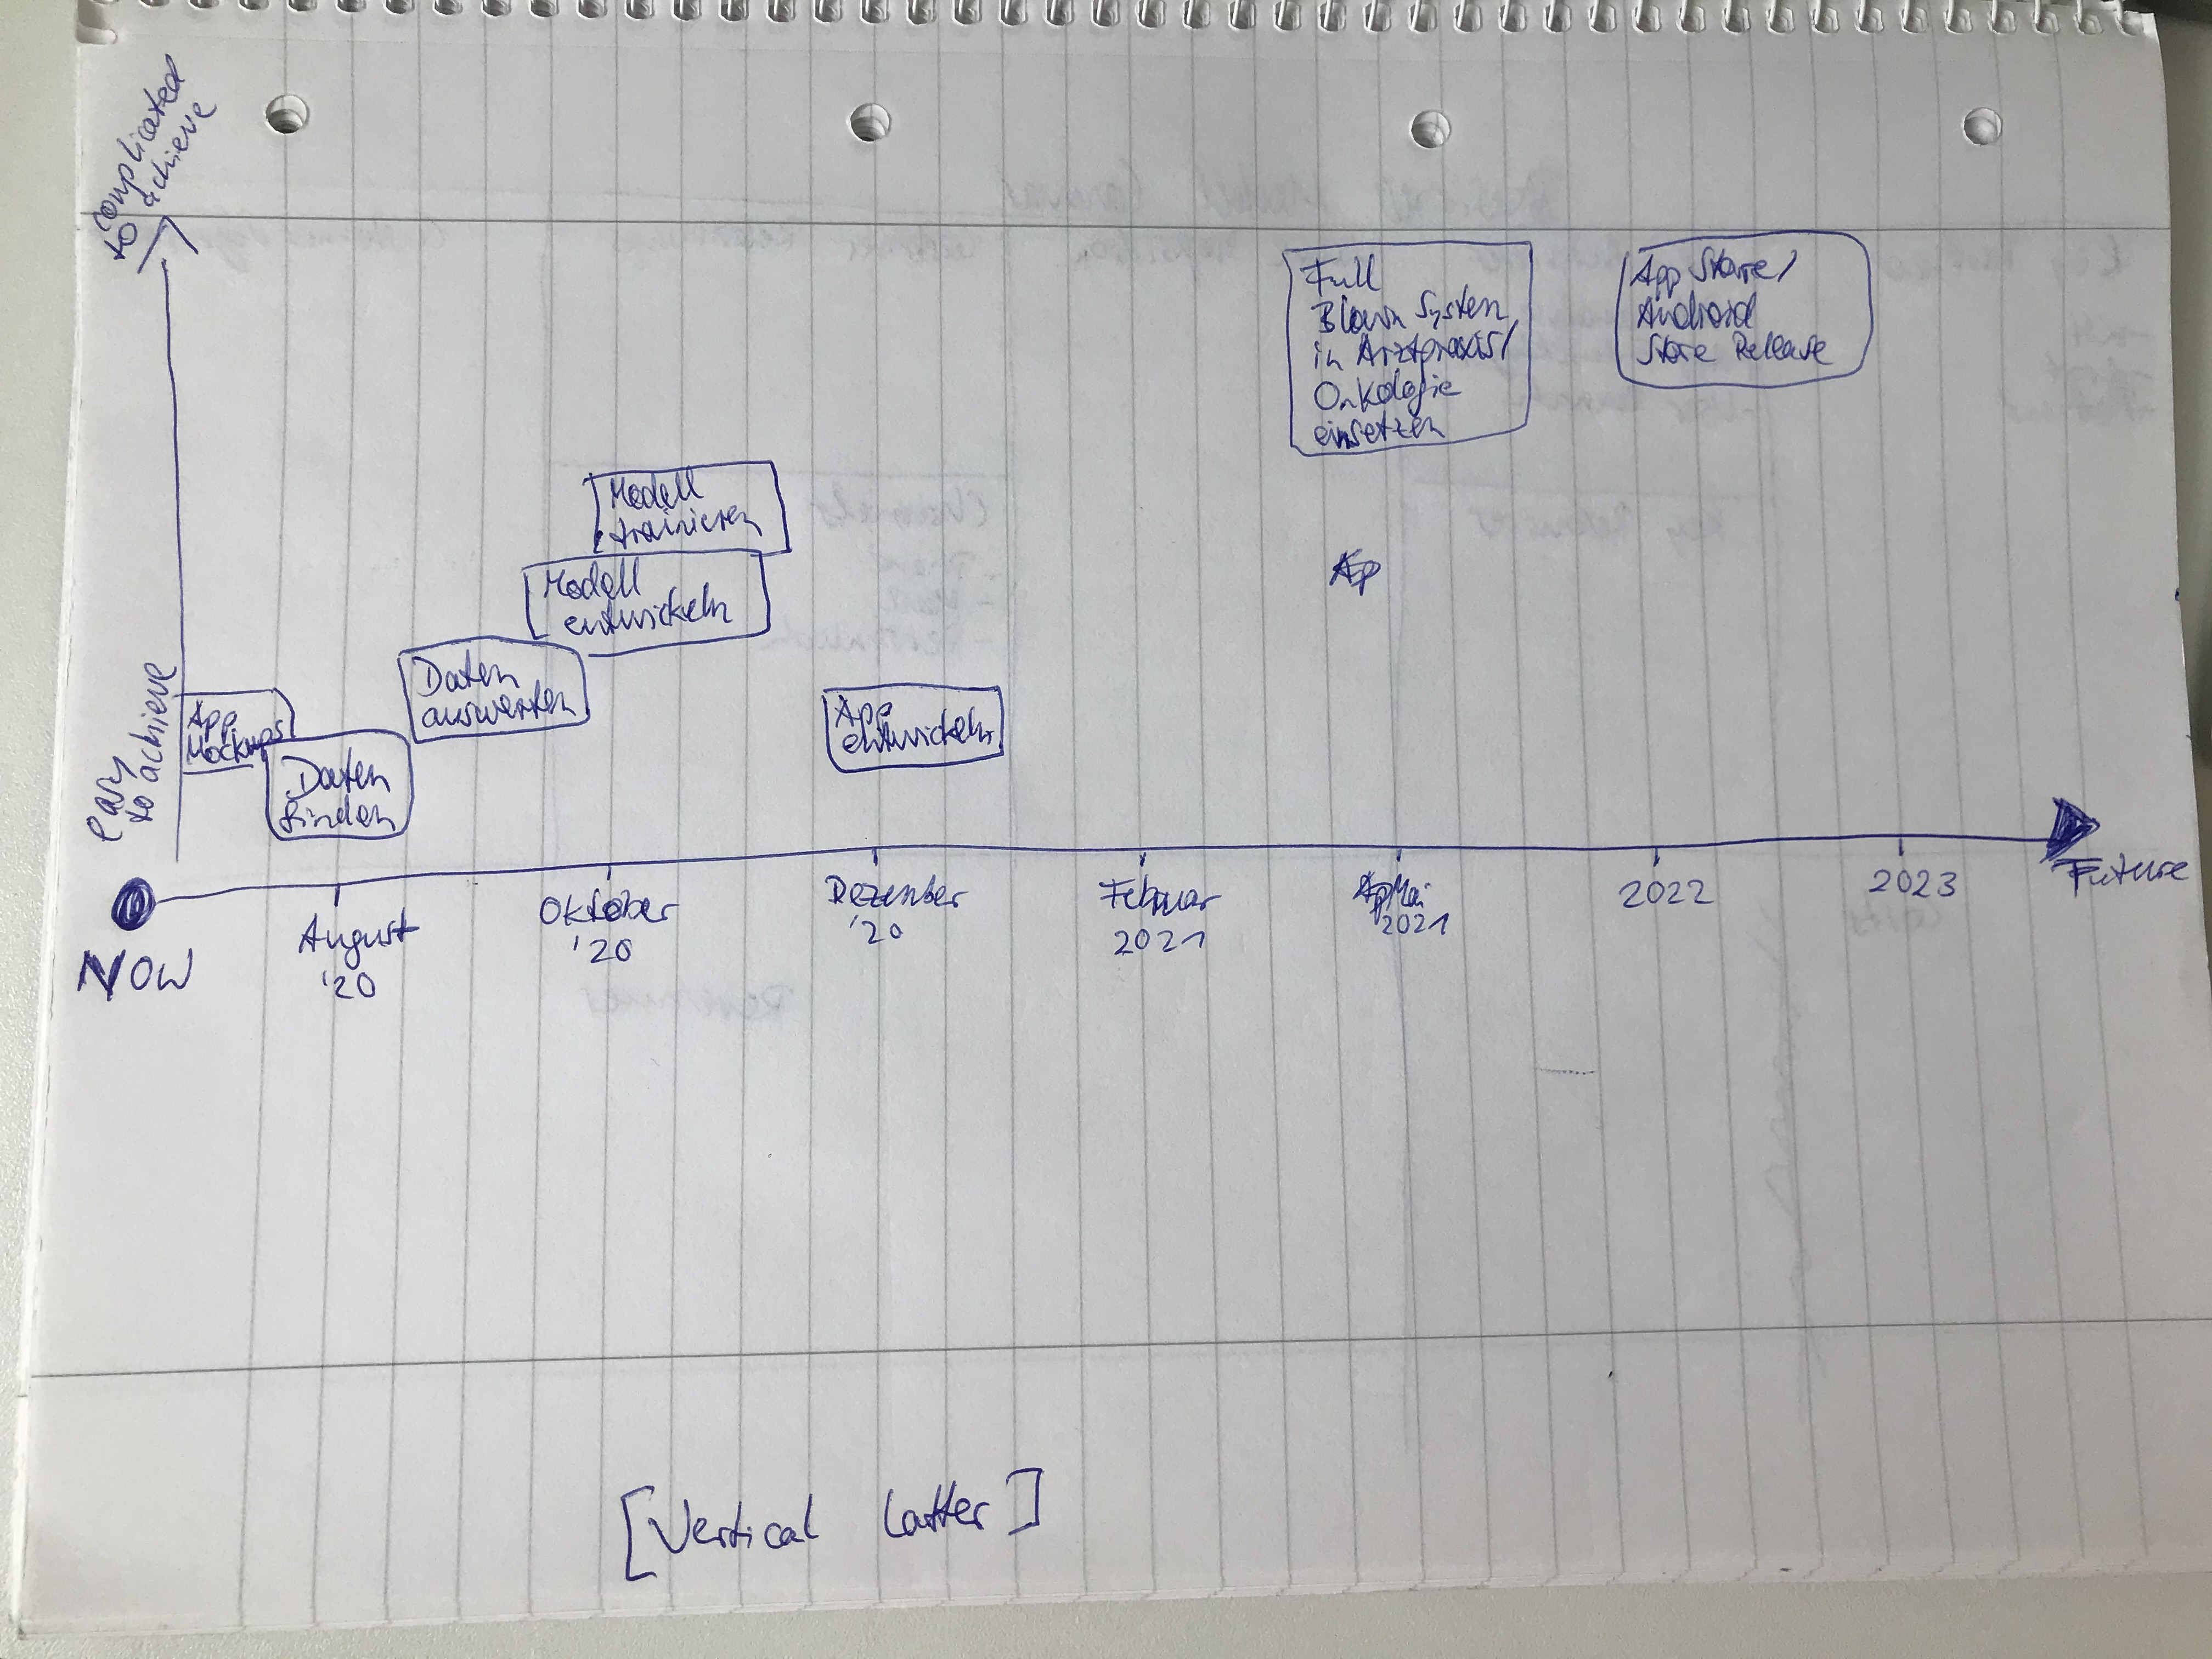
\includegraphics[width=1\textwidth]{images/verticallatter.jpg}
	\caption{Vertical latter which defines the development goals over time}
	\label{verticallatter}
\end{figure}

\subsection{How might we?}

\begin{figure}[h!]
	\centering
	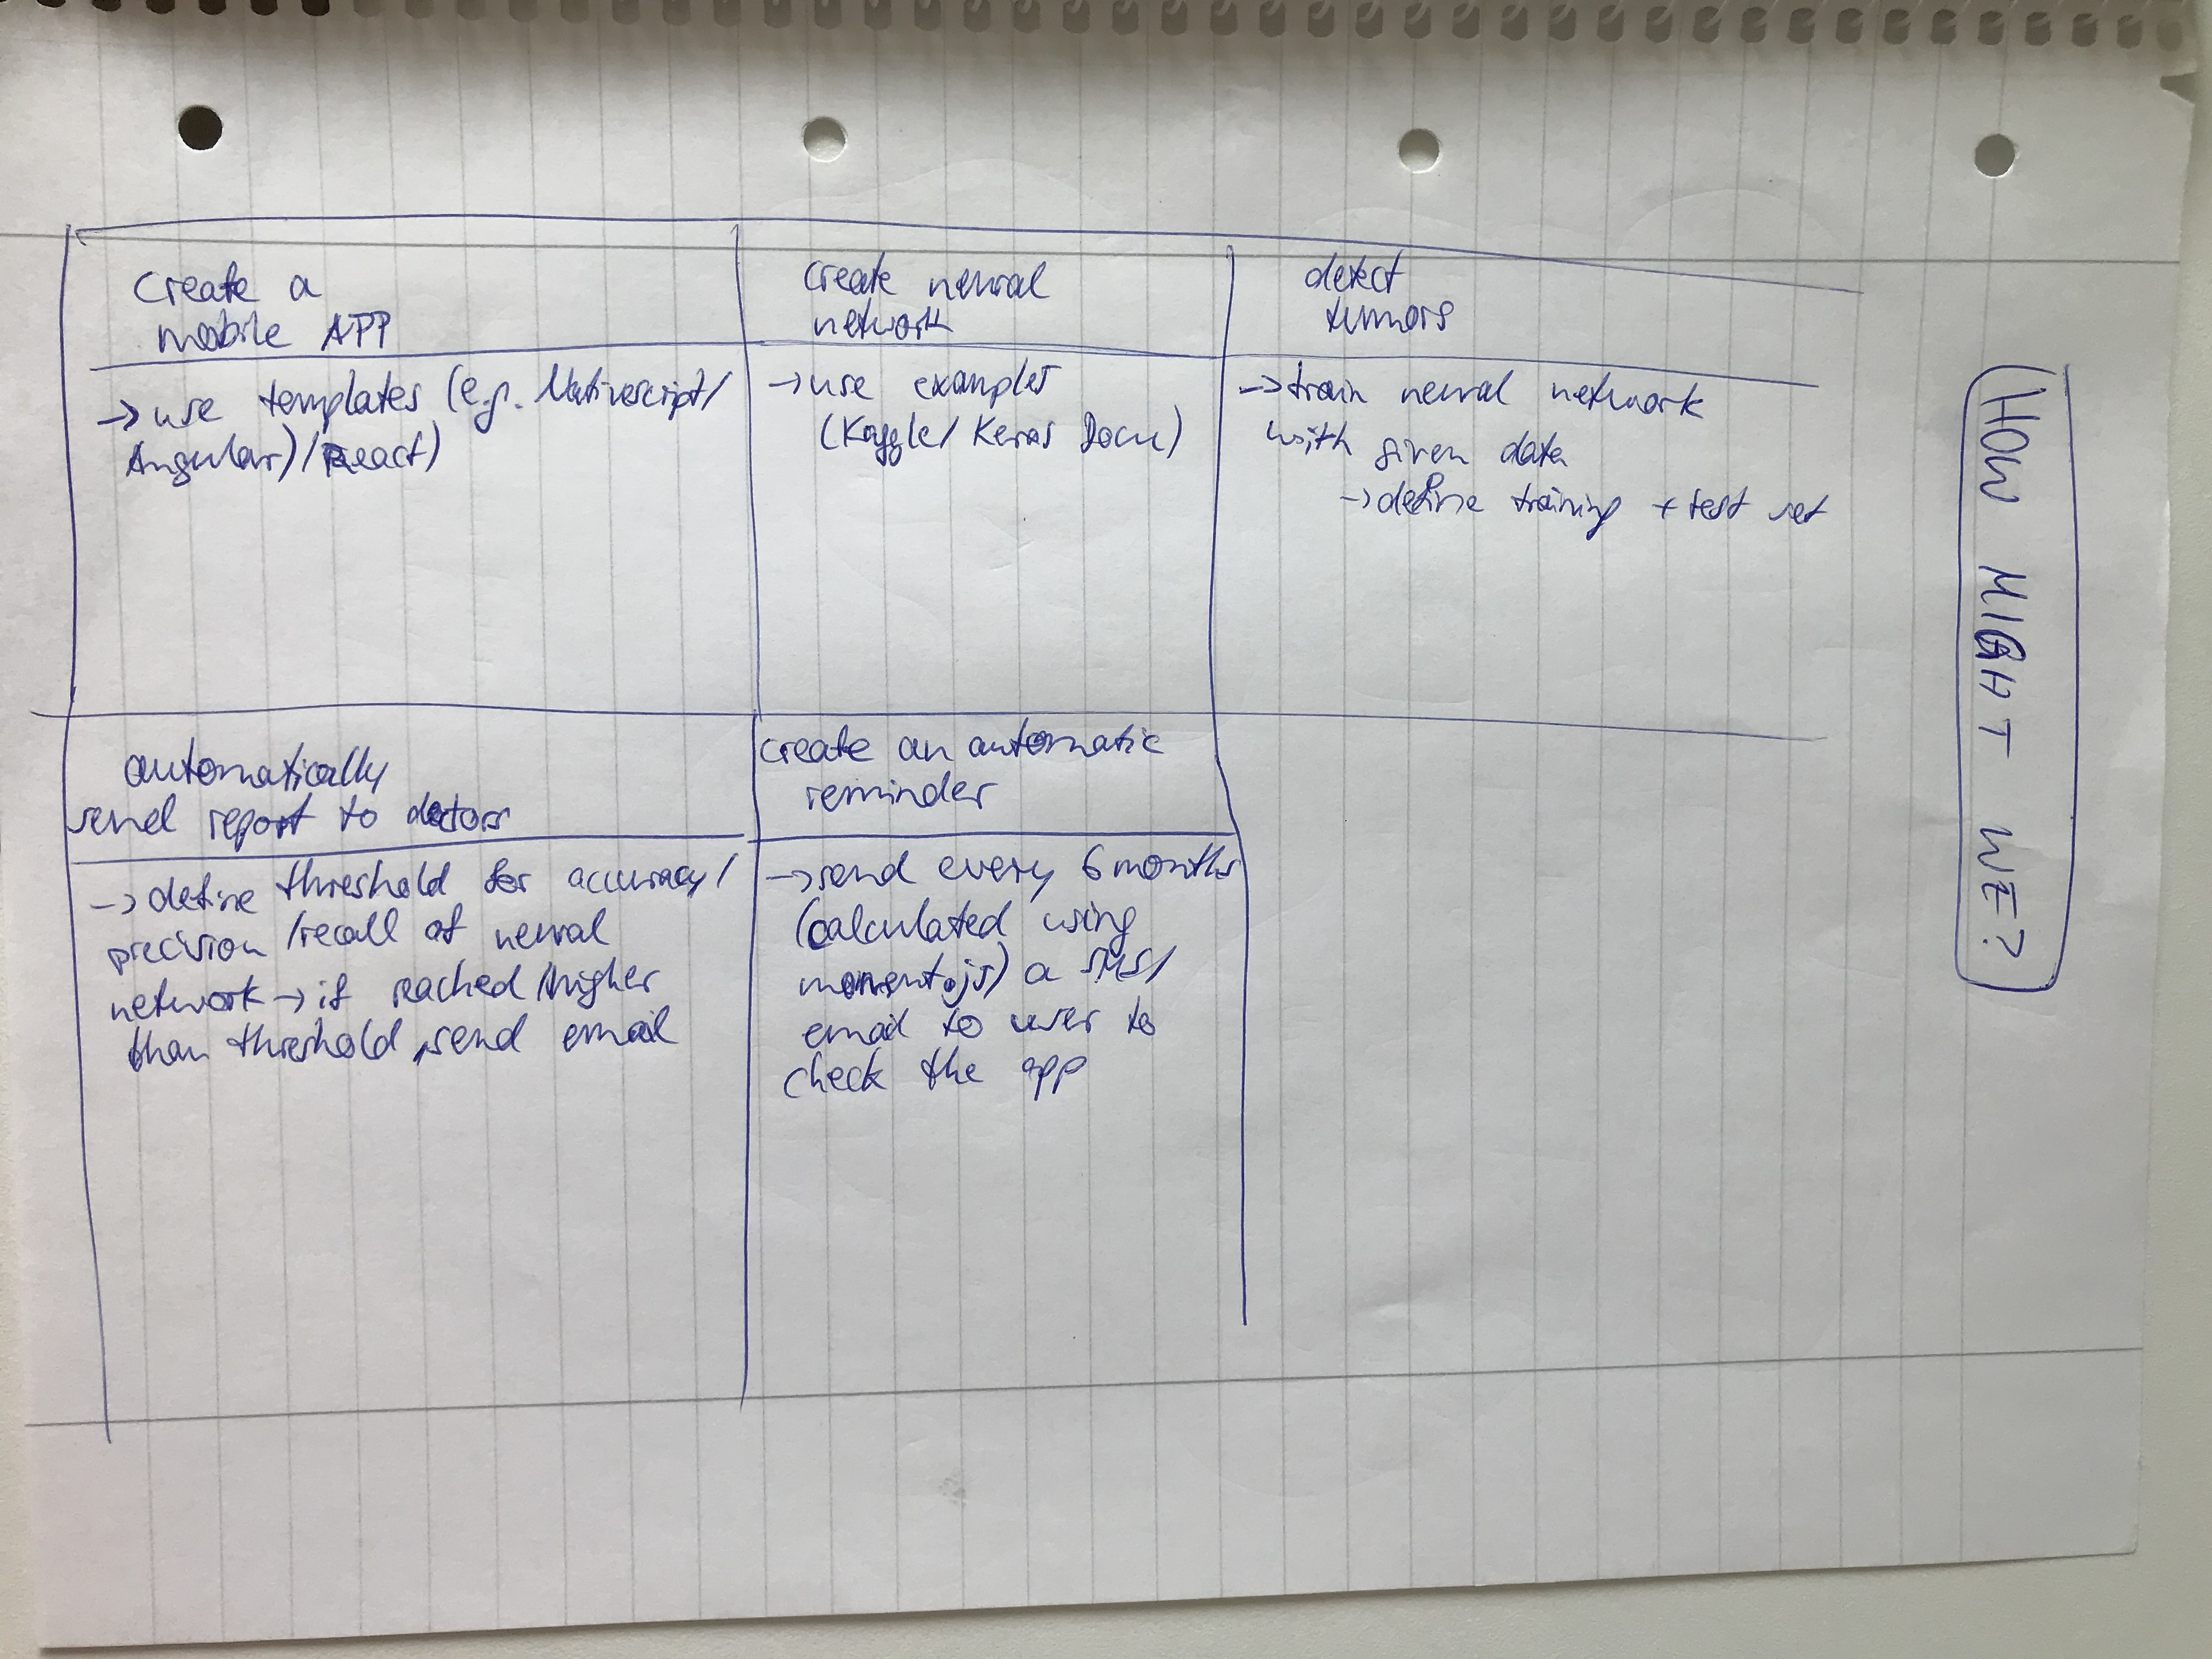
\includegraphics[width=1\textwidth]{images/howmightwe.jpg}
	\caption{"How might we?" - table to define the process of development}
	\label{howmightwe}
\end{figure}

\subsection{Stakeholder Map}

Figure \ref{stakeholdermap} gives an overview of potential stakeholders. As can be seen in this figure, there are four groups of users: patients, doctors, the IT appartment of the hospital and the 

\begin{figure}[h!]
	\centering
	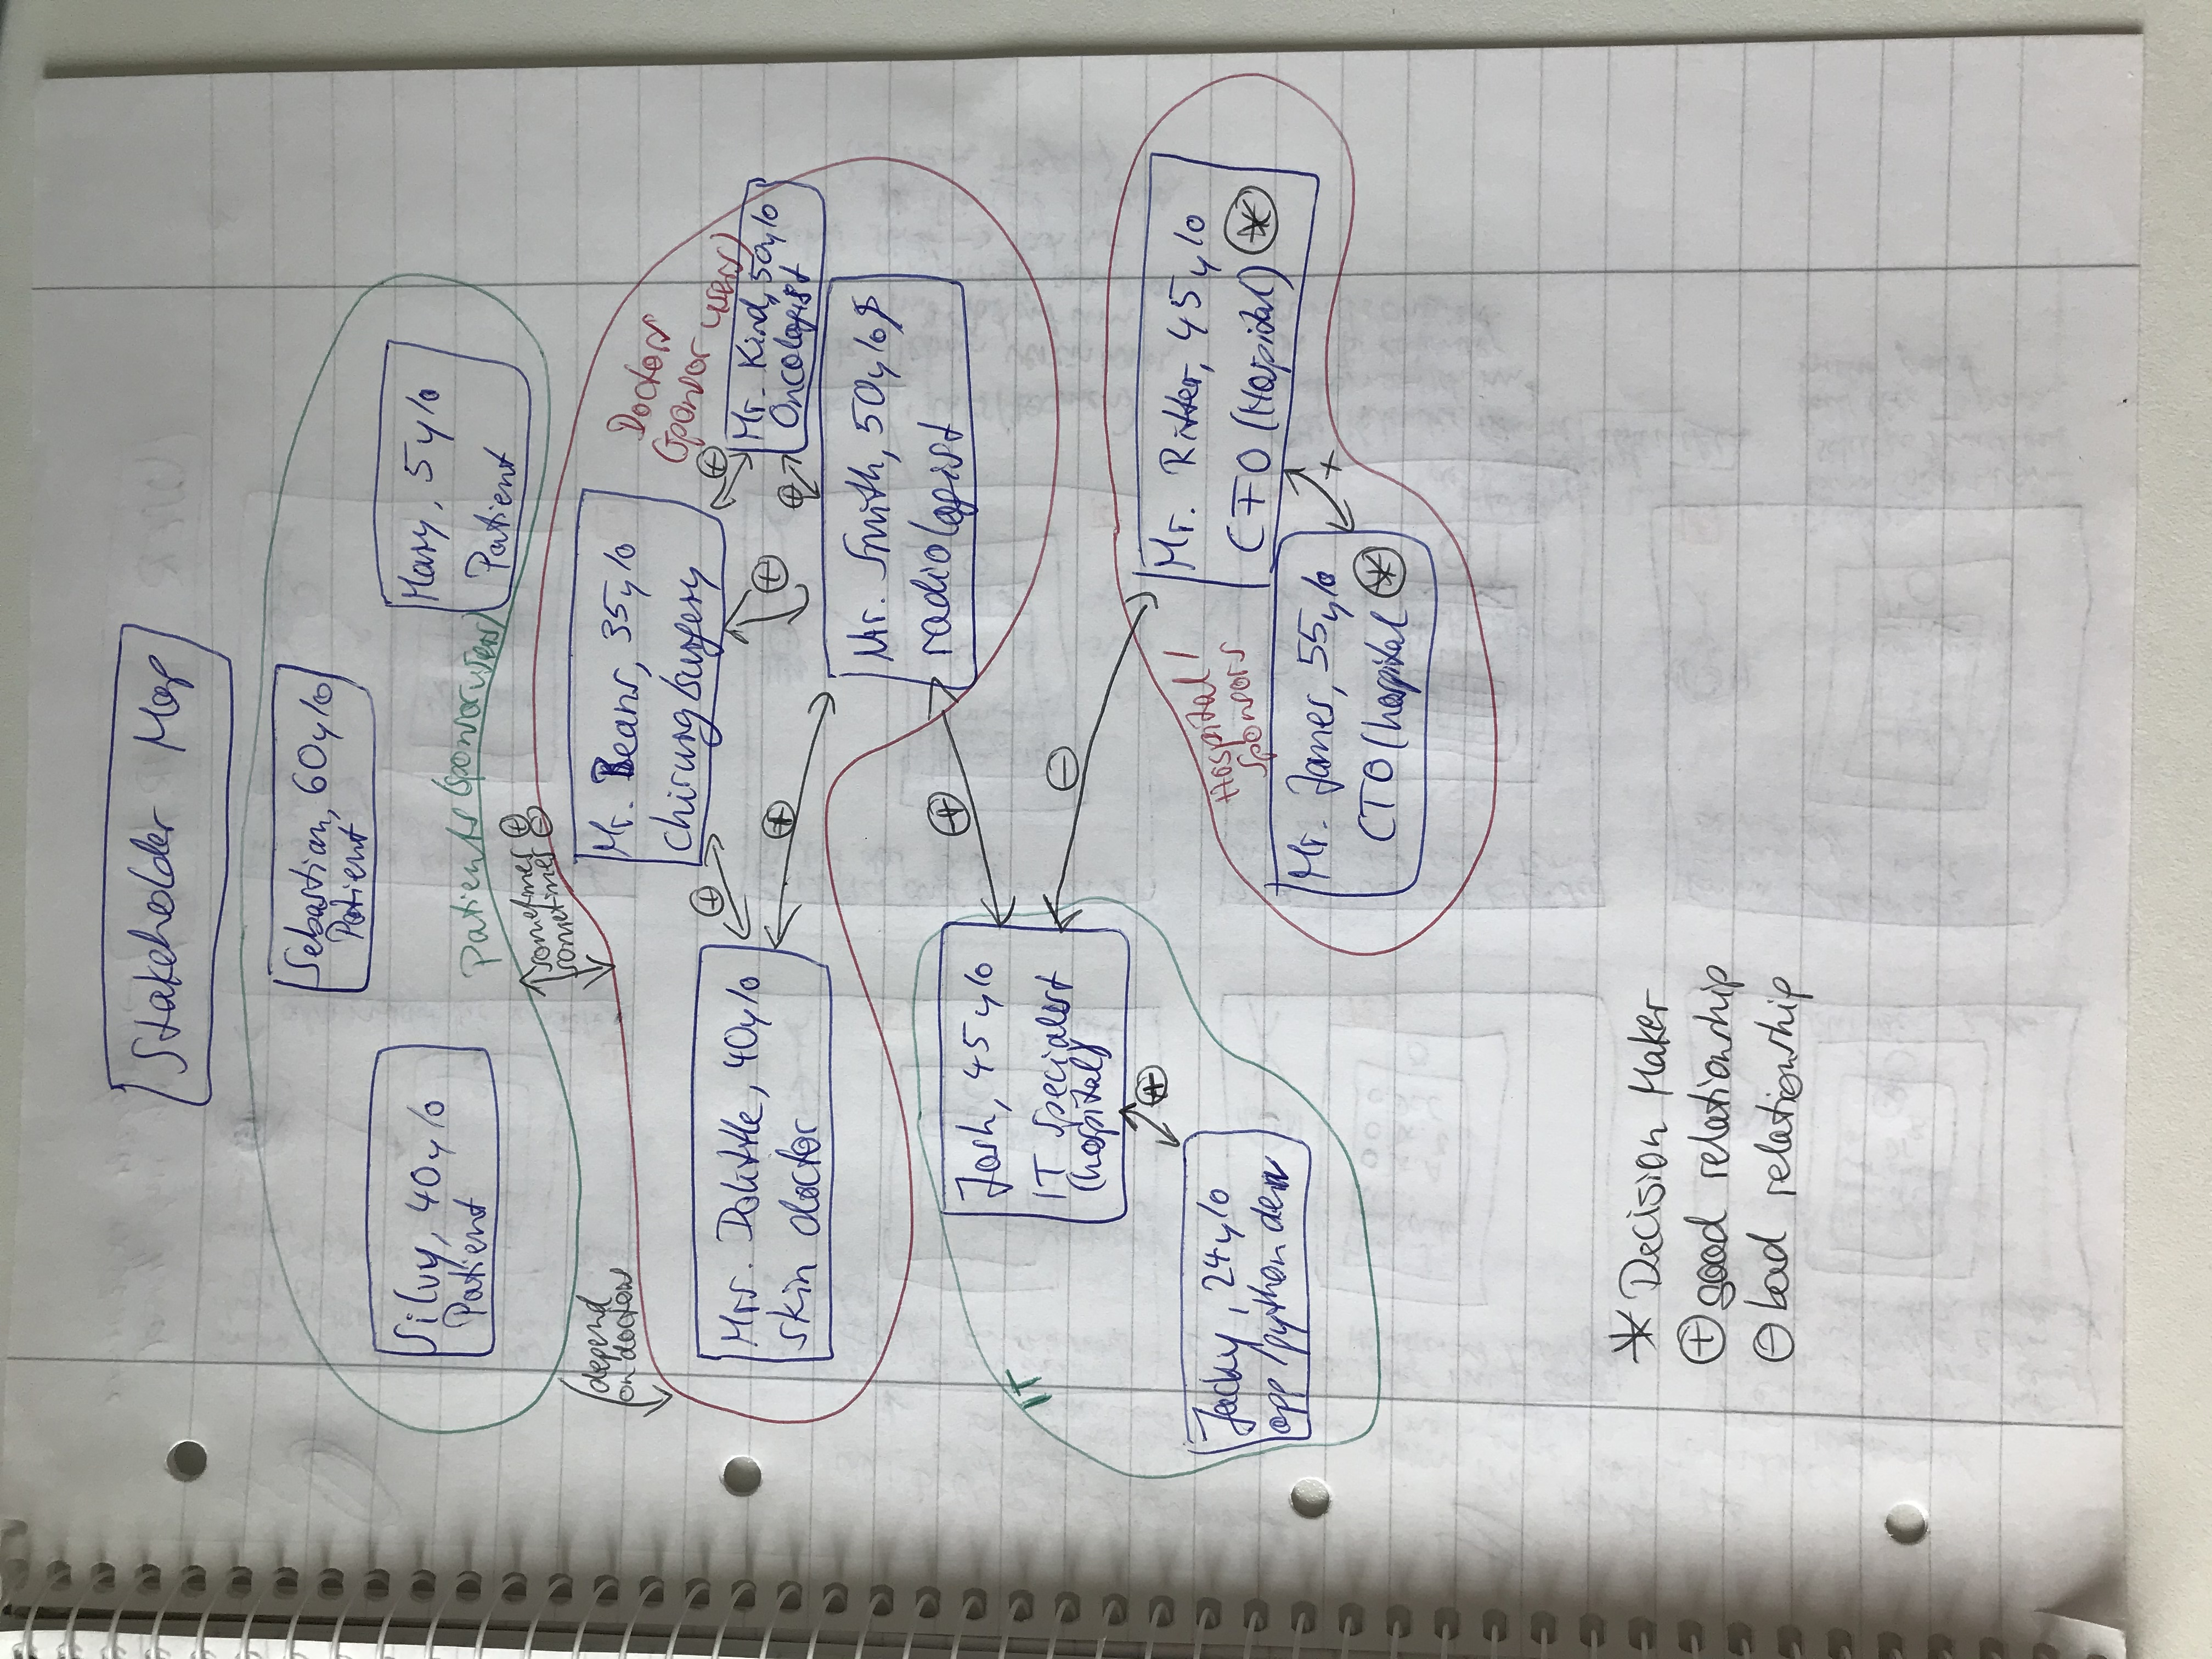
\includegraphics[width=1\textwidth]{images/stakeholdermap.jpg}
	\caption{Stakeholder Map which shows all groups of stakeholders as well as their relationships}
	\label{stakeholdermap}
\end{figure}

\subsection{Empathy Map}

In this section, three primary developed persona were developed. They should represent each of them a specific user of the user groups. Figures \ref{radiologist}, \ref{patient}, \ref{cfo} give an overview of what each persona feels and thinks about the treatment process of cancer, especially skin cancer. Moreover, the empathy maps were developed before asking affected patients and might differ from real opinions. But during the first step of this project this method serves well to specify the business case. 

\begin{figure}[h!]
	\centering
	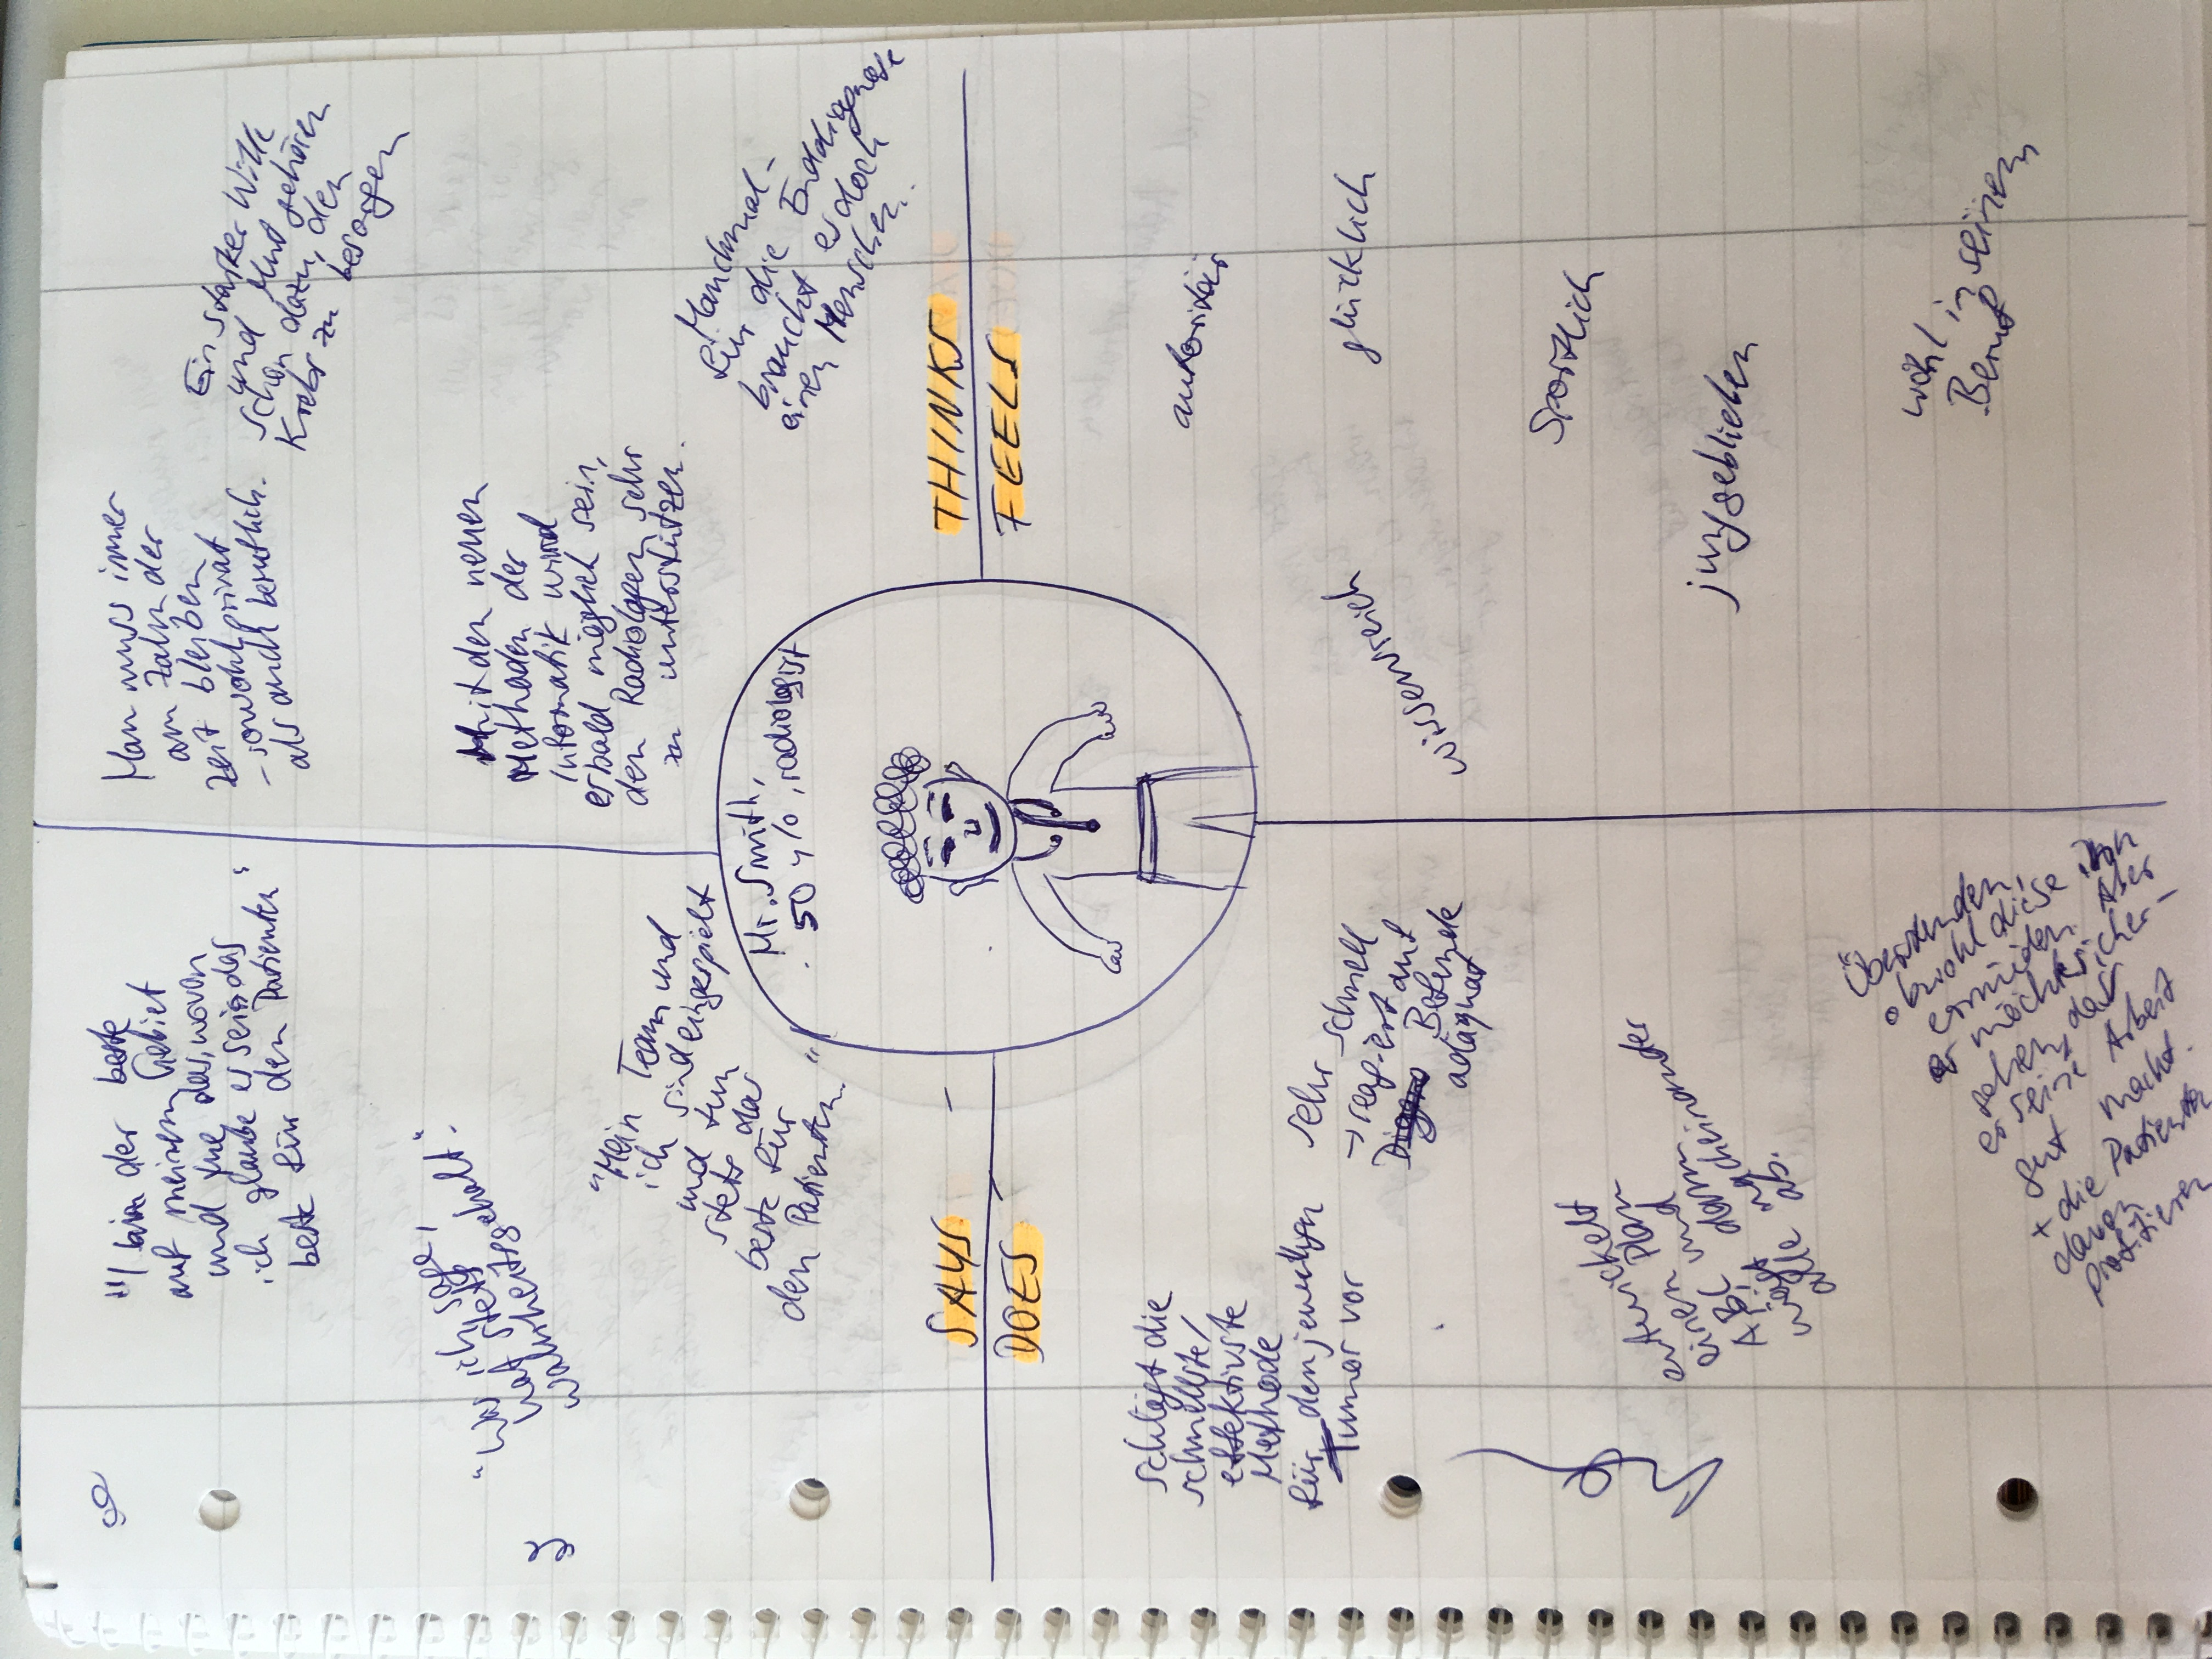
\includegraphics[width=1\textwidth]{images/empathymap_radiologist.jpg}
	\caption{Empathy Map of radiologist}
	\label{radiologist}
\end{figure}

\begin{figure}[h!]
	\centering
	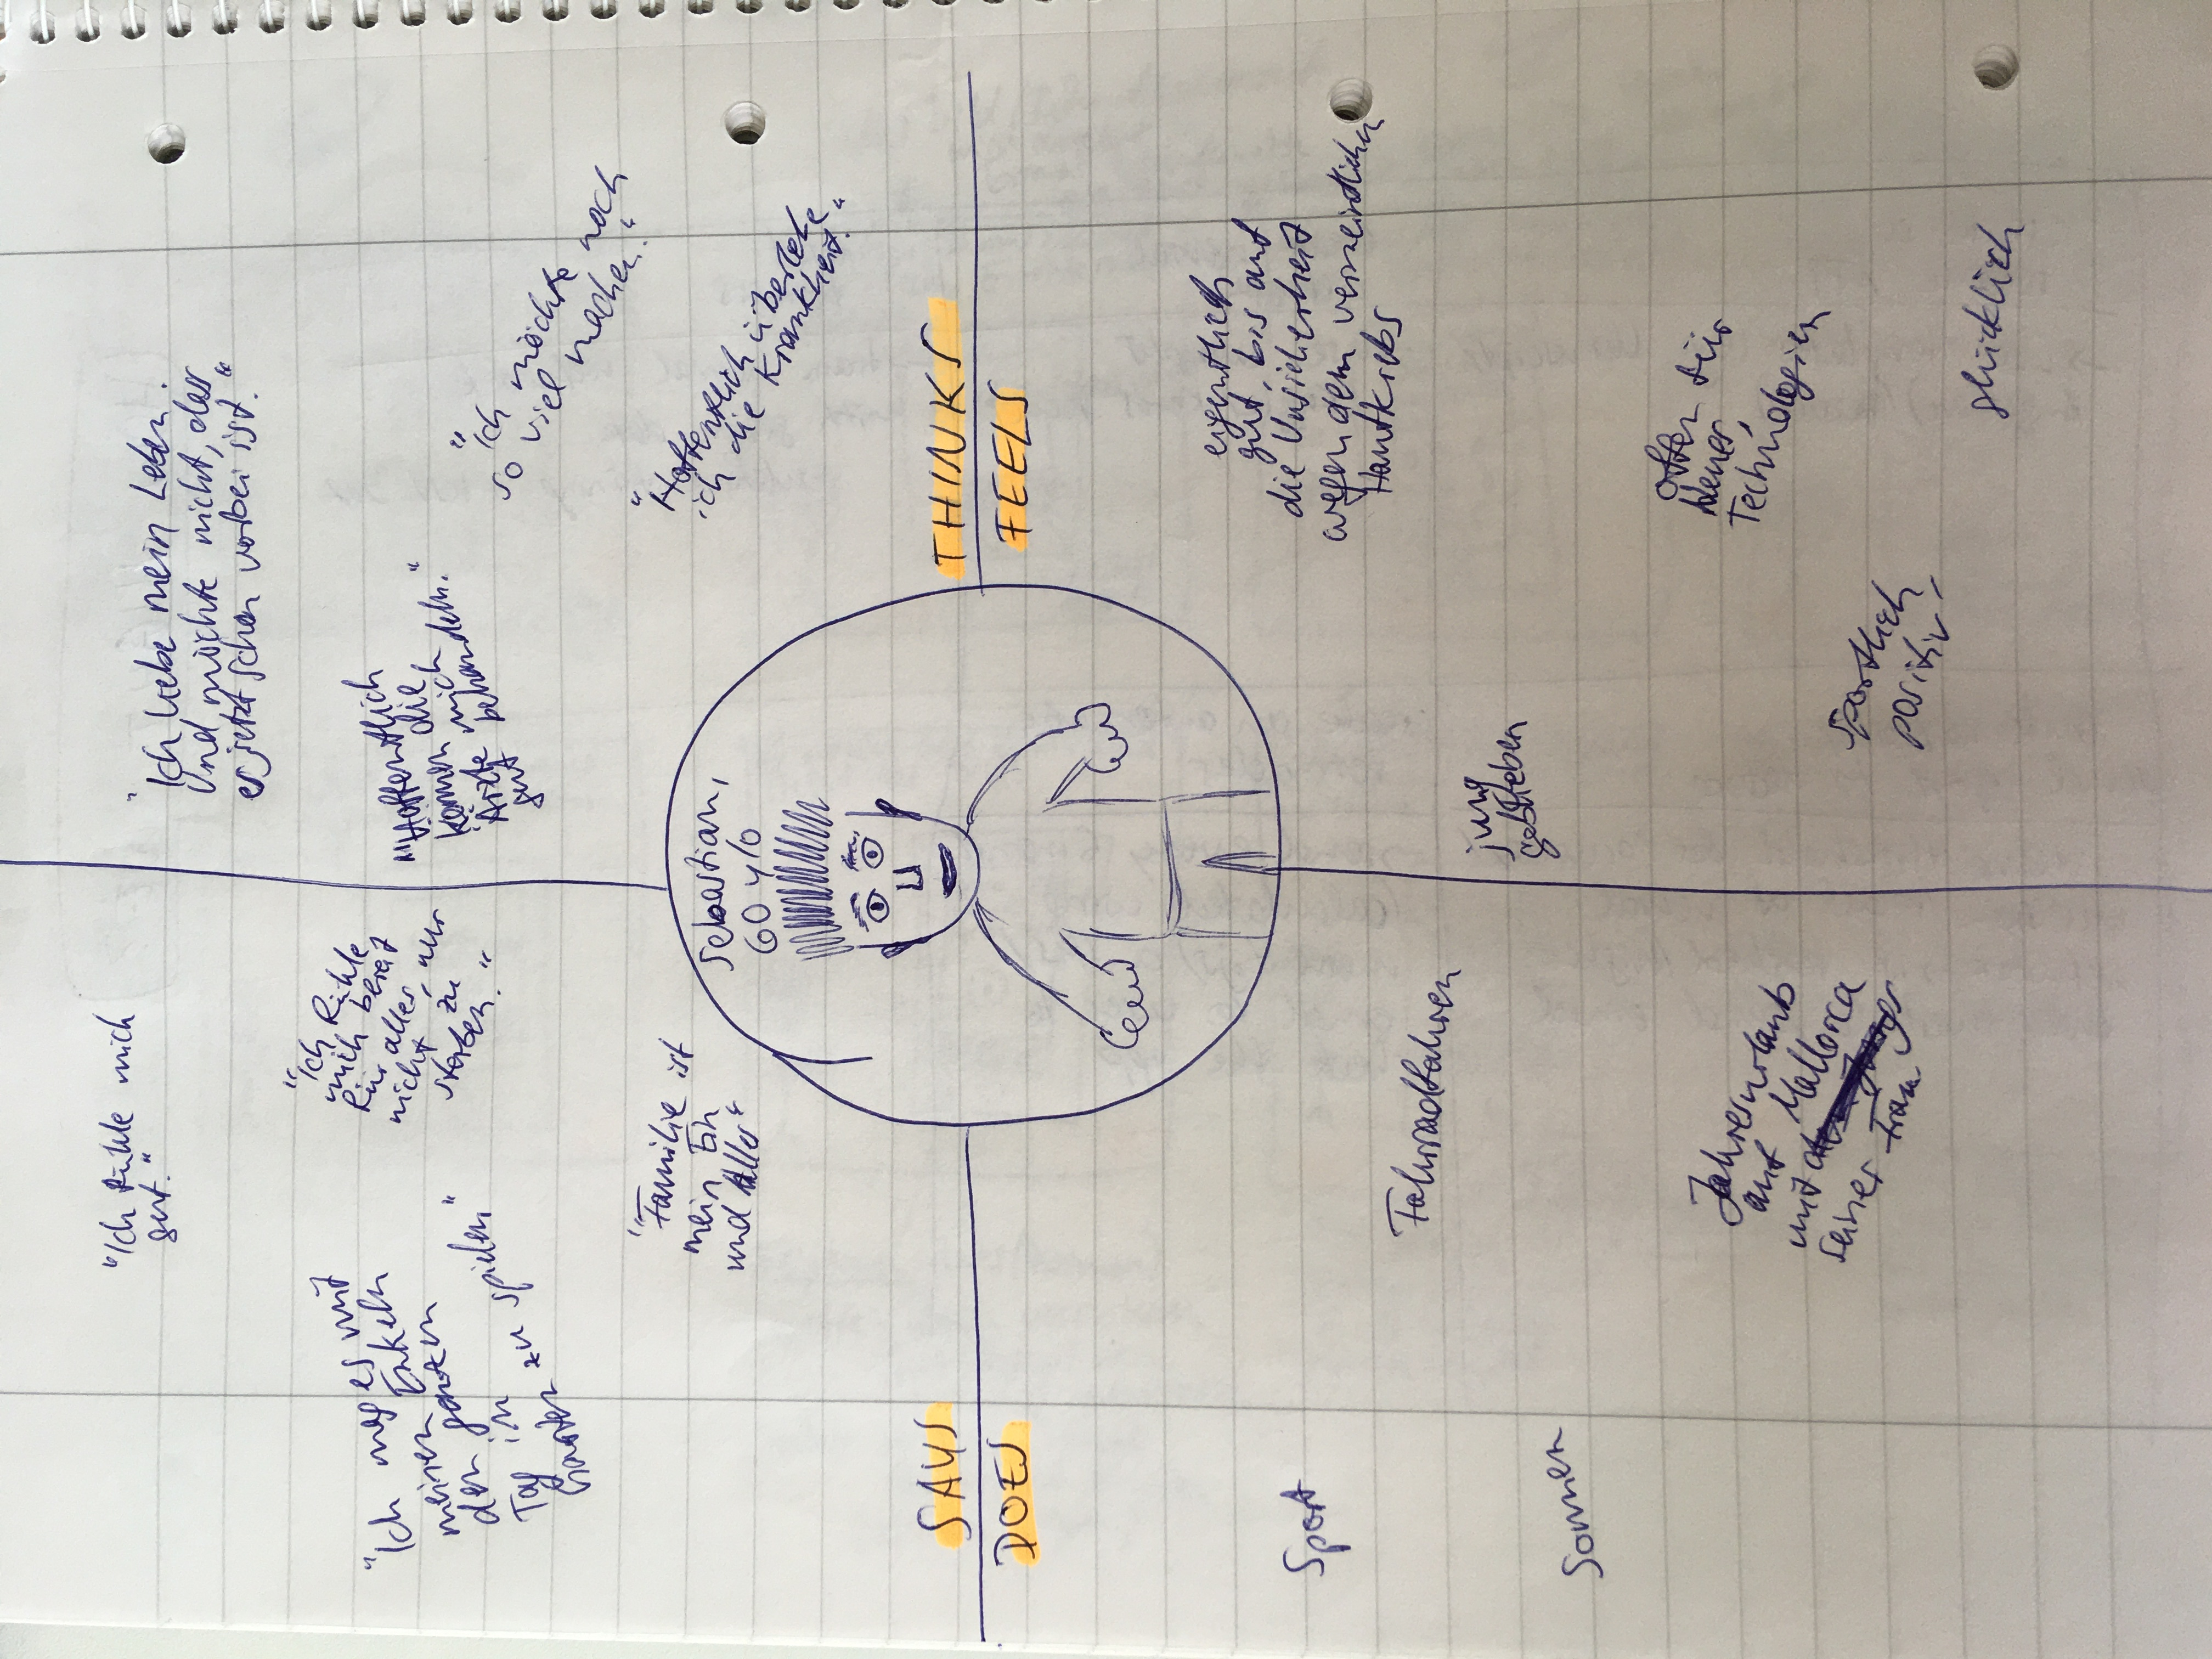
\includegraphics[width=1\textwidth]{images/empathymap_patient.jpg}
	\caption{Empathy Map of patient}
	\label{patient}
\end{figure}

\begin{figure}[h!]
	\centering
	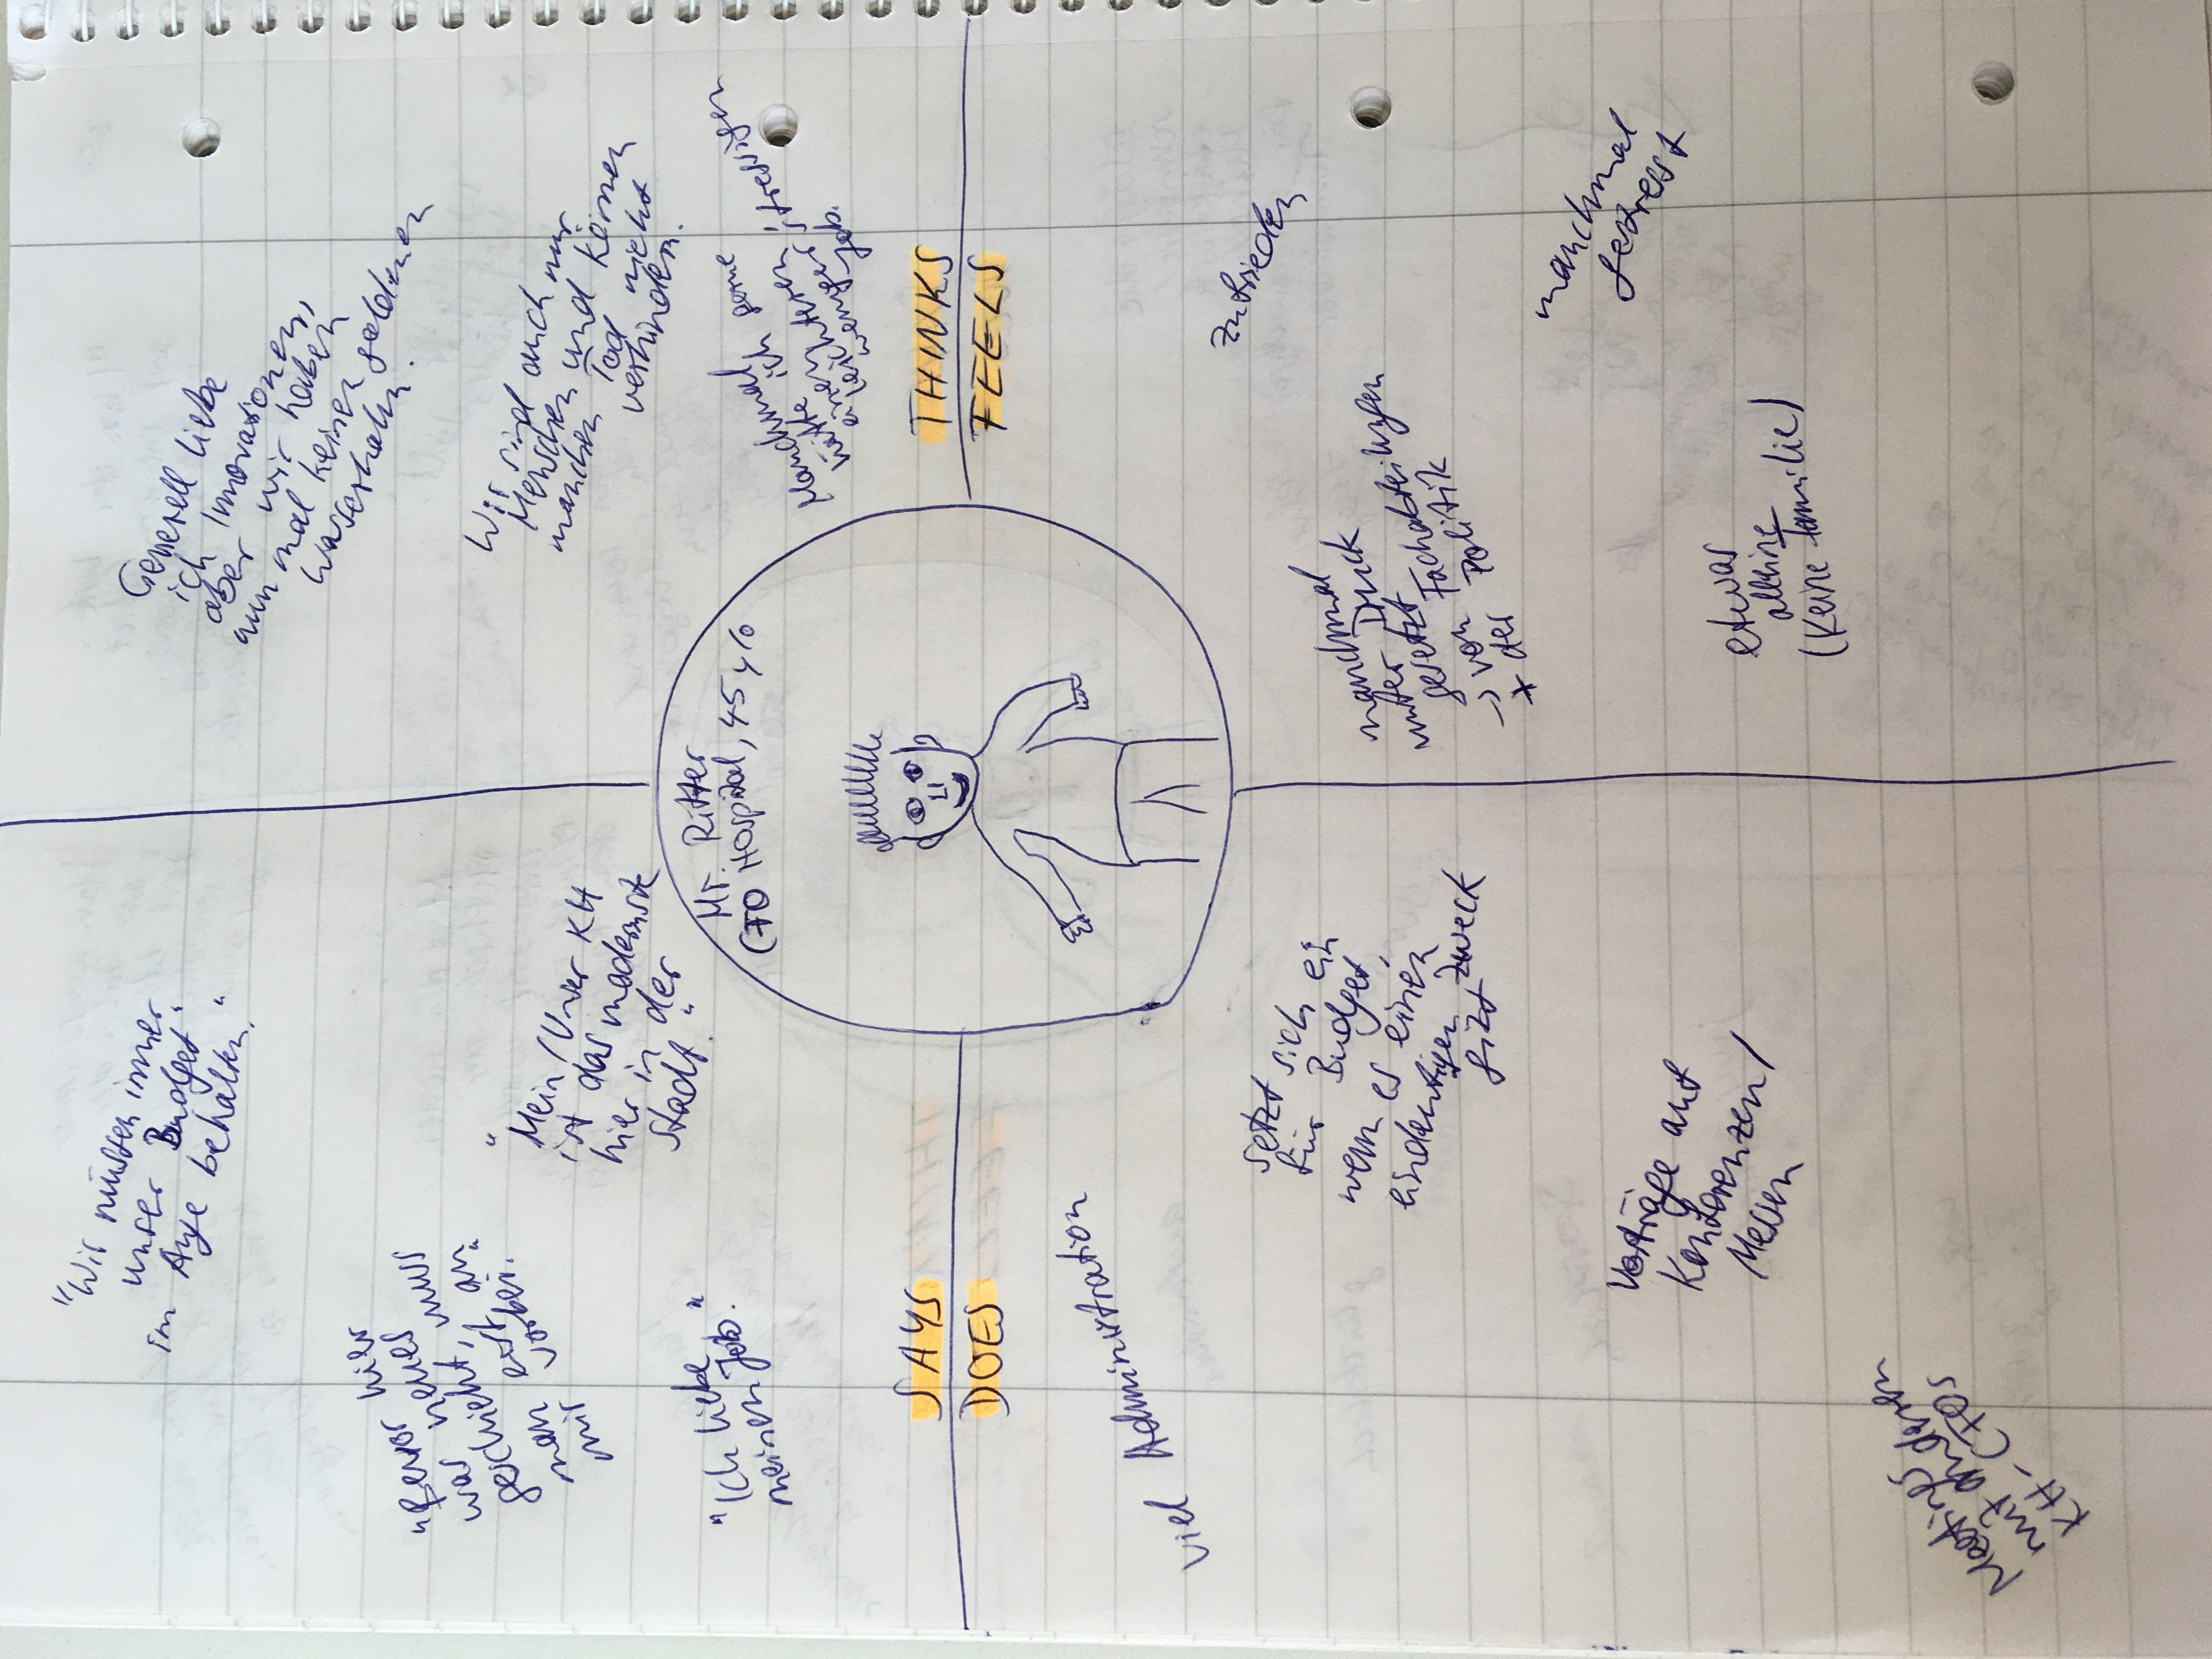
\includegraphics[width=1\textwidth]{images/empathymap_cfo.jpg}
	\caption{Empathy Map of \ac{cfo} of hospital}
	\label{cfo}
\end{figure}


\subsection{Hills}

The design thinking method "hills" is a special method to prioritize the real needs of users and to set special goals that differ the solution from existing apps. The second fact is really important for development. As this method answers the three questions 'WHO', 'WHAT' and 'HOW'\footnote{\cite{ibm_edt}}, the focus is on the most important feature which shall be realized. In further planning, this feature can be divided into multiple 'todos'  during development process. This raises the practicability of the product and accelerates the development. Figure \ref{hills} shows the developed hills which explain two different point of views: On the one hand, patient's view and on the otherhand, the doctor's view.
To give an example, one hill is expressed as: 'As a patient, i would like to have a reliable, real-time and easy-to-understand diagnose about my type of skin cancer.'
Another hill is: 'As a doctor, i would like the application to outline potential skin tumors and to calculate the  approximate amount of medication and how it has to be administered. Furthermore, there should be a check whether the medication is available at the hospital's pharmacy or not. If the medication is not available, it should be ordered immediately and delivered to the patient.

\begin{figure}[h!]
	\centering
	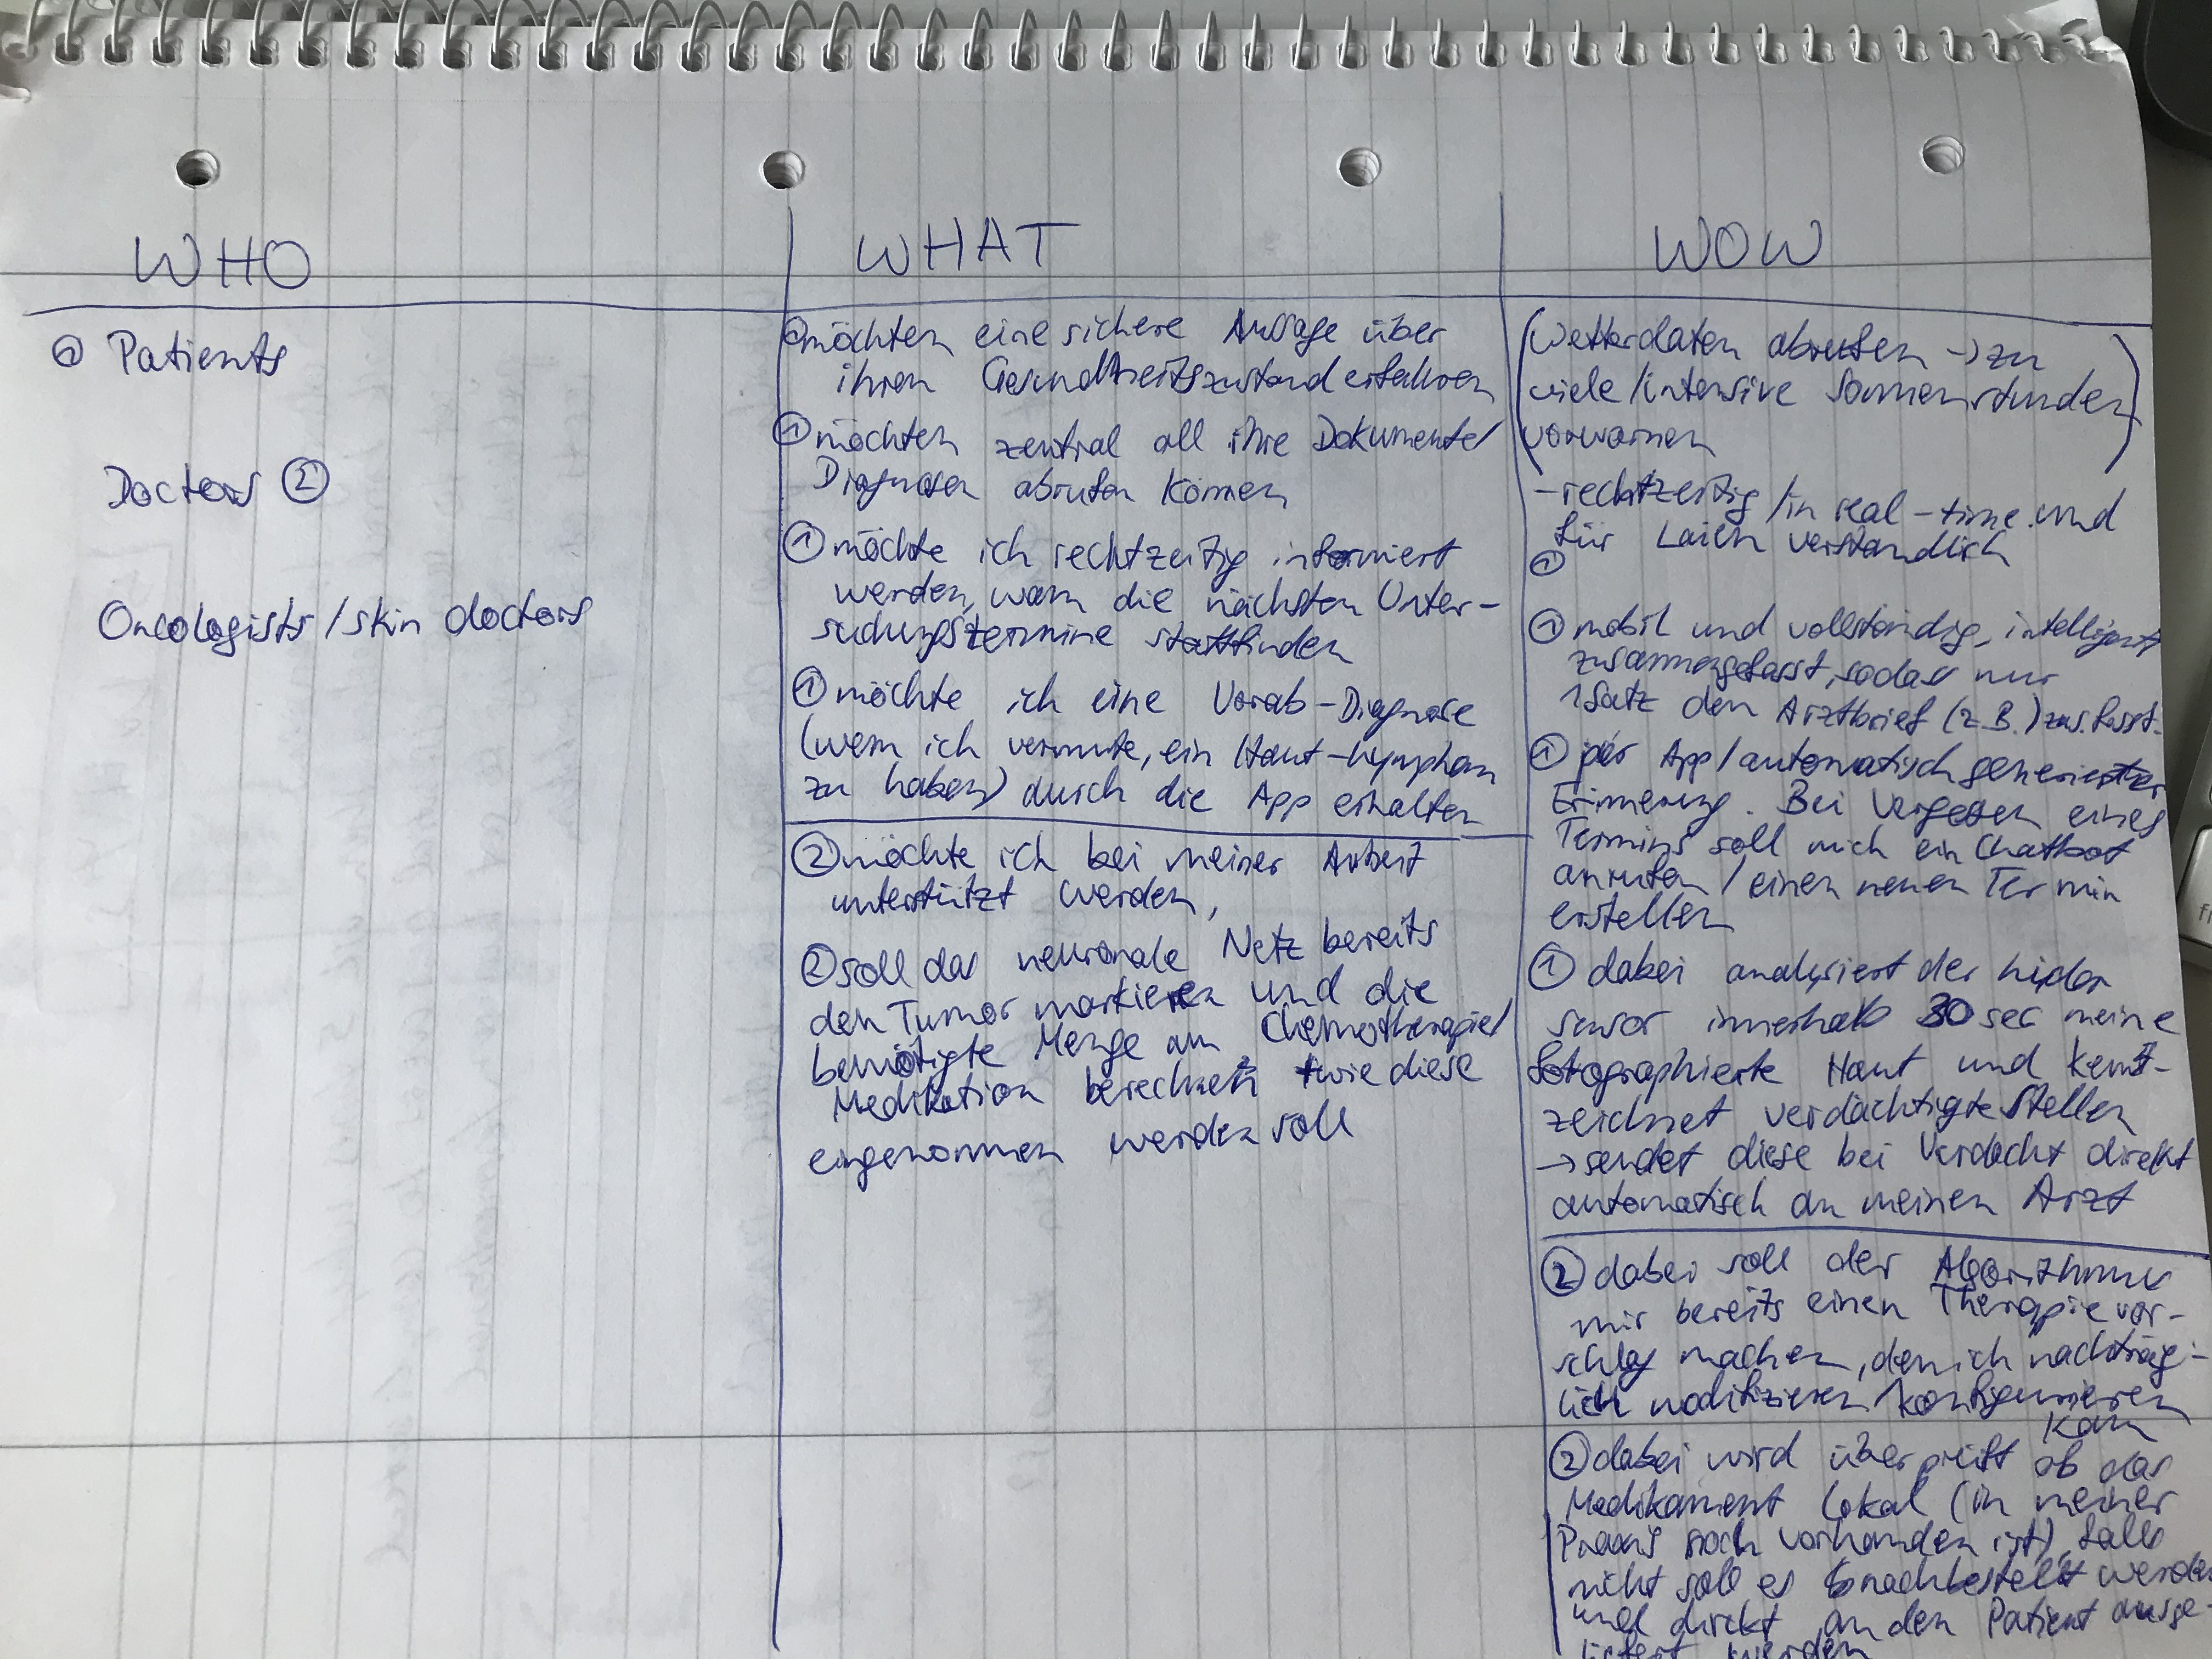
\includegraphics[width=1\textwidth]{images/hills.jpg}
	\caption{"How might we?" - table to define the process of development}
	\label{hills}
\end{figure}

\subsection{User Journey}

\begin{figure}[h!]
	\centering
	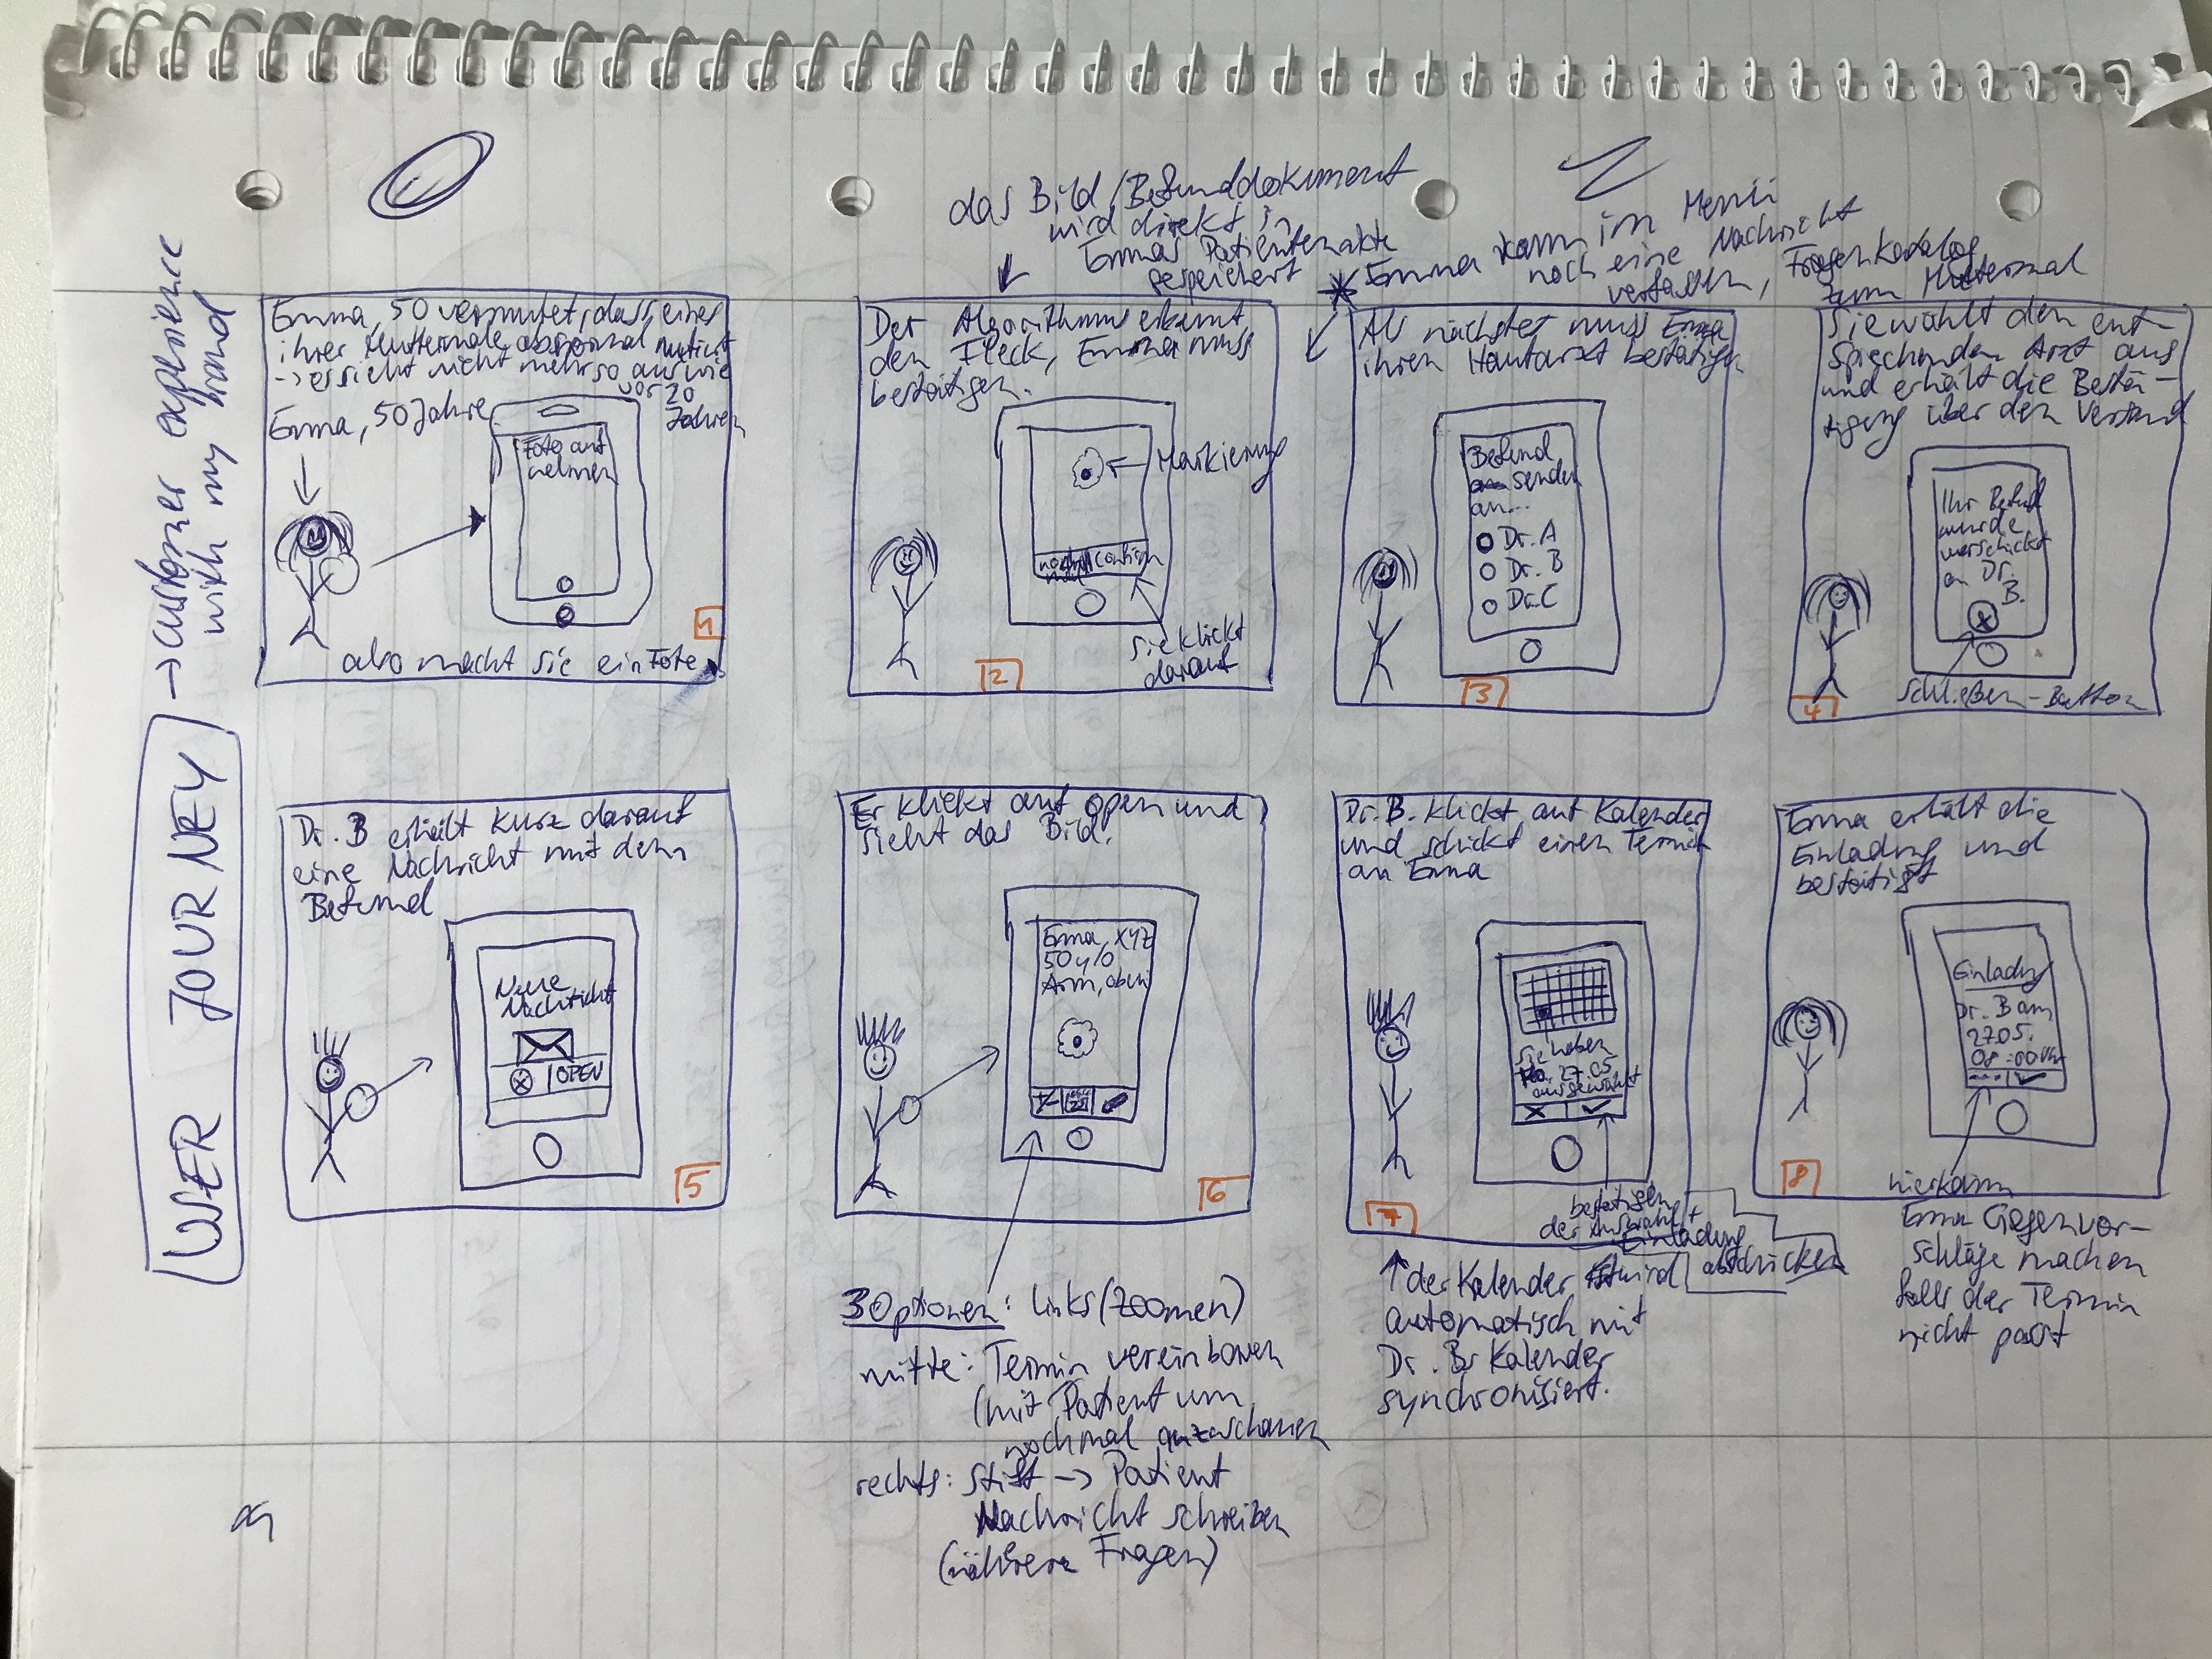
\includegraphics[width=1\textwidth]{images/userjourney.jpg}
	\caption{User Journey which describes the interaction of key users and app}
	\label{verticallatter}
\end{figure}

\section{User Research}
\subsection{User interviews}
\subsection{What is important? - Relevant features}
\subsection{How can processes be improved?}


\section{Development of system to predict metastasis and recidives} 

\subsection{Challenges of development}
Concerning the detection of skin moles are tattoos, skin lesions and tone of skin. In a first approach, these were not considered. But for future development, the usage of Lidar\footnote{\cite{czichos_introduction_2018}} sensor could be a solution. Since Lidar detects the 3D model of an object by calculating the distance from the detecting camera to the patient's skin, some special moles can be distinguished. 

\subsection{Data Research}
\paragraph{Kaggle dataset}
For training and developing the neural network, a basic Kaggle dataset was used \footnote{\cite{kaggle_dataset}}. It contains 3600 pictures of skin moles with the format 224x244 px. These 3600 files are divided into benign and malignant skin moles. 
For training, the neural network has to learn how to distinguish good from bad tumors and then set a warning. 
The dataset contains both training and test data. Since these are not labeled, in the first step, data preprocessing, labels have to be created.

\subsection{\ac{crisp-dm}: Model Planning and Learning}

\subsection{U-net architecture to for medical imaging}
A recent approach to detect tumors or objects that were marked by doctors in order to train a neural network is called 'U-Net Architecture' \footnote{\cite{unet}}. It is a \ac{cnn} architecture to 'fast and precise segment objects in images'.
Figure XY gives an impression of a simple U-Net. 
'Each blue box corresponds to a multi-channel feature map. The number of channels is denoted on top of the box. The x-y-size is provided at the lower left edge of the box. White boxes represent copied feature maps. The arrows denote the different operations.'\footnote{\cite{unet}}
One of the advantages is that during the first step (going right and downwards), objects are detected and in the second step (going right and upwards) the precise localization of the objects is calculated. 

\begin{figure}[h!]
	\centering
	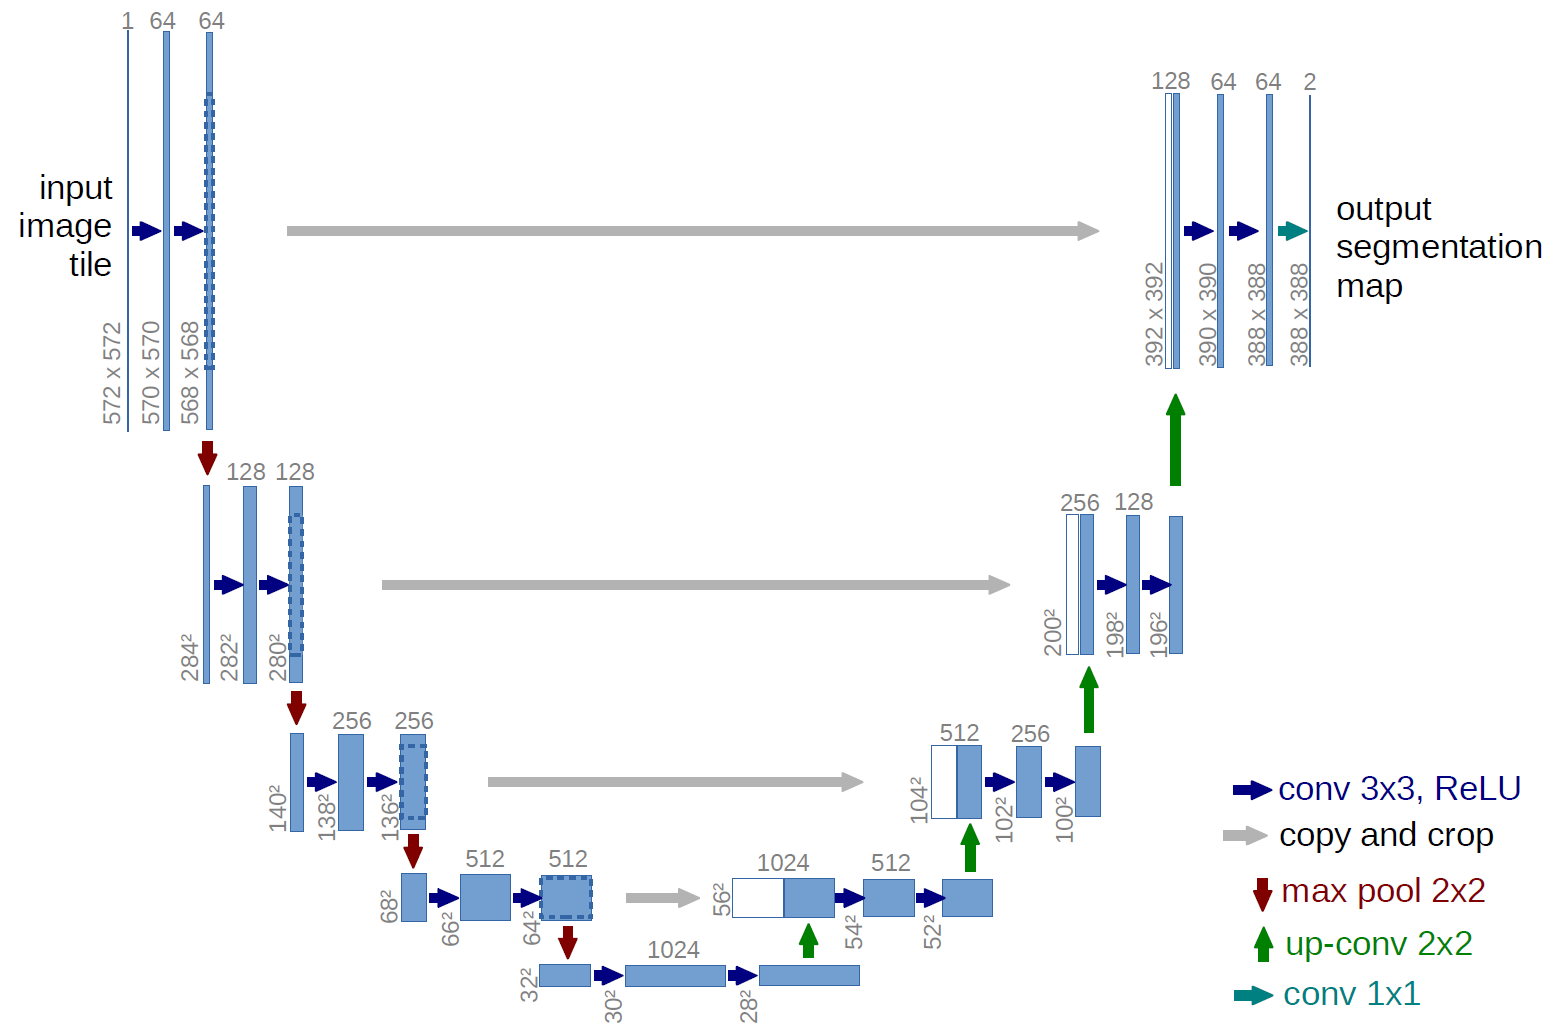
\includegraphics[width=1\textwidth]{images/u-net-architecture.png}
	\caption{U-Net architecture (example for 32x32 pixels in the lowest resolution)}
	\label{unet}
\end{figure}

According to Ronneberger et al.\footnote{\cite{unet_freiburg}}, U-Net learns segmentation in an end-to-end setting. Furthermore, very few annotated images (approximately 30 per application) are needed. Touching objects of the same class.

\subsection{Testing}
\subsection{Results} 

\chapter{Results}
\section{Validation of results}
\section{Limitation in the development process}

\chapter{Conclusion and Outlook}
\section{Conclusion}
\section{Outlook}


\chapter{Abbreviations}
\begin{acronym}[CRISP-DM]
\acro{crisp-dm}[CRISP-DM]{CRoss-Industry Standard Process for Data Mining}
\acro{cfo}[CFO]{Chief Financial Officer}
\acro{who}[WHO]{World Health Organization}
\acro{iarc}[IARC]{International Agency for Research on Cancer}
\acro{ham10000}[HAM10000]{Human Against Machine with 10000 training images}
\end{acronym}

\printbibliography[heading=bibintoc]

\chapter{Appendix A}\label{appendix a}
\ohead[]{Ehrenwörtliche Erklärung \hfill \thepage}

\null\vfill
\textbf{Ehrenwörtliche Erklärung}

Hiermit versichere ich, dass die vorliegende Arbeit von mir selbstständig und ohne unerlaubte Hilfe angefertigt worden ist, insbesondere dass ich alle Stellen, die wörtlich oder annähernd wörtlich aus Veröffentlichungen entnommen sind, durch Zitate als solche gekennzeichnet habe. Ich versichere auch, dass die von mir eingereichte schriftliche Version mit der digitalen Version übereinstimmt. Weiterhin erkläre ich, dass die Arbeit in gleicher oder ähnlicher Form noch keiner Prüfungsbehörde / Prüfungsstelle vorgelegen hat. Ich erkläre mich damit nicht einverstanden, dass die Arbeit der Öffentlichkeit zugänglich gemacht wird. Ich erkläre mich damit einverstanden, dass die Digitalversion dieser Arbeit zwecks Plagiatsprüfung auf die Server externer Anbieter hochgeladen werden darf. Die Plagiatsprüfung stellt keine Zurverfügungstellung für die Öffentlichkeit dar.

\ \\ \ \\ 


Ort, Datum (Vorname Nachname)

\vfill
%\chapter{Appendix B}\label{appendix b}
%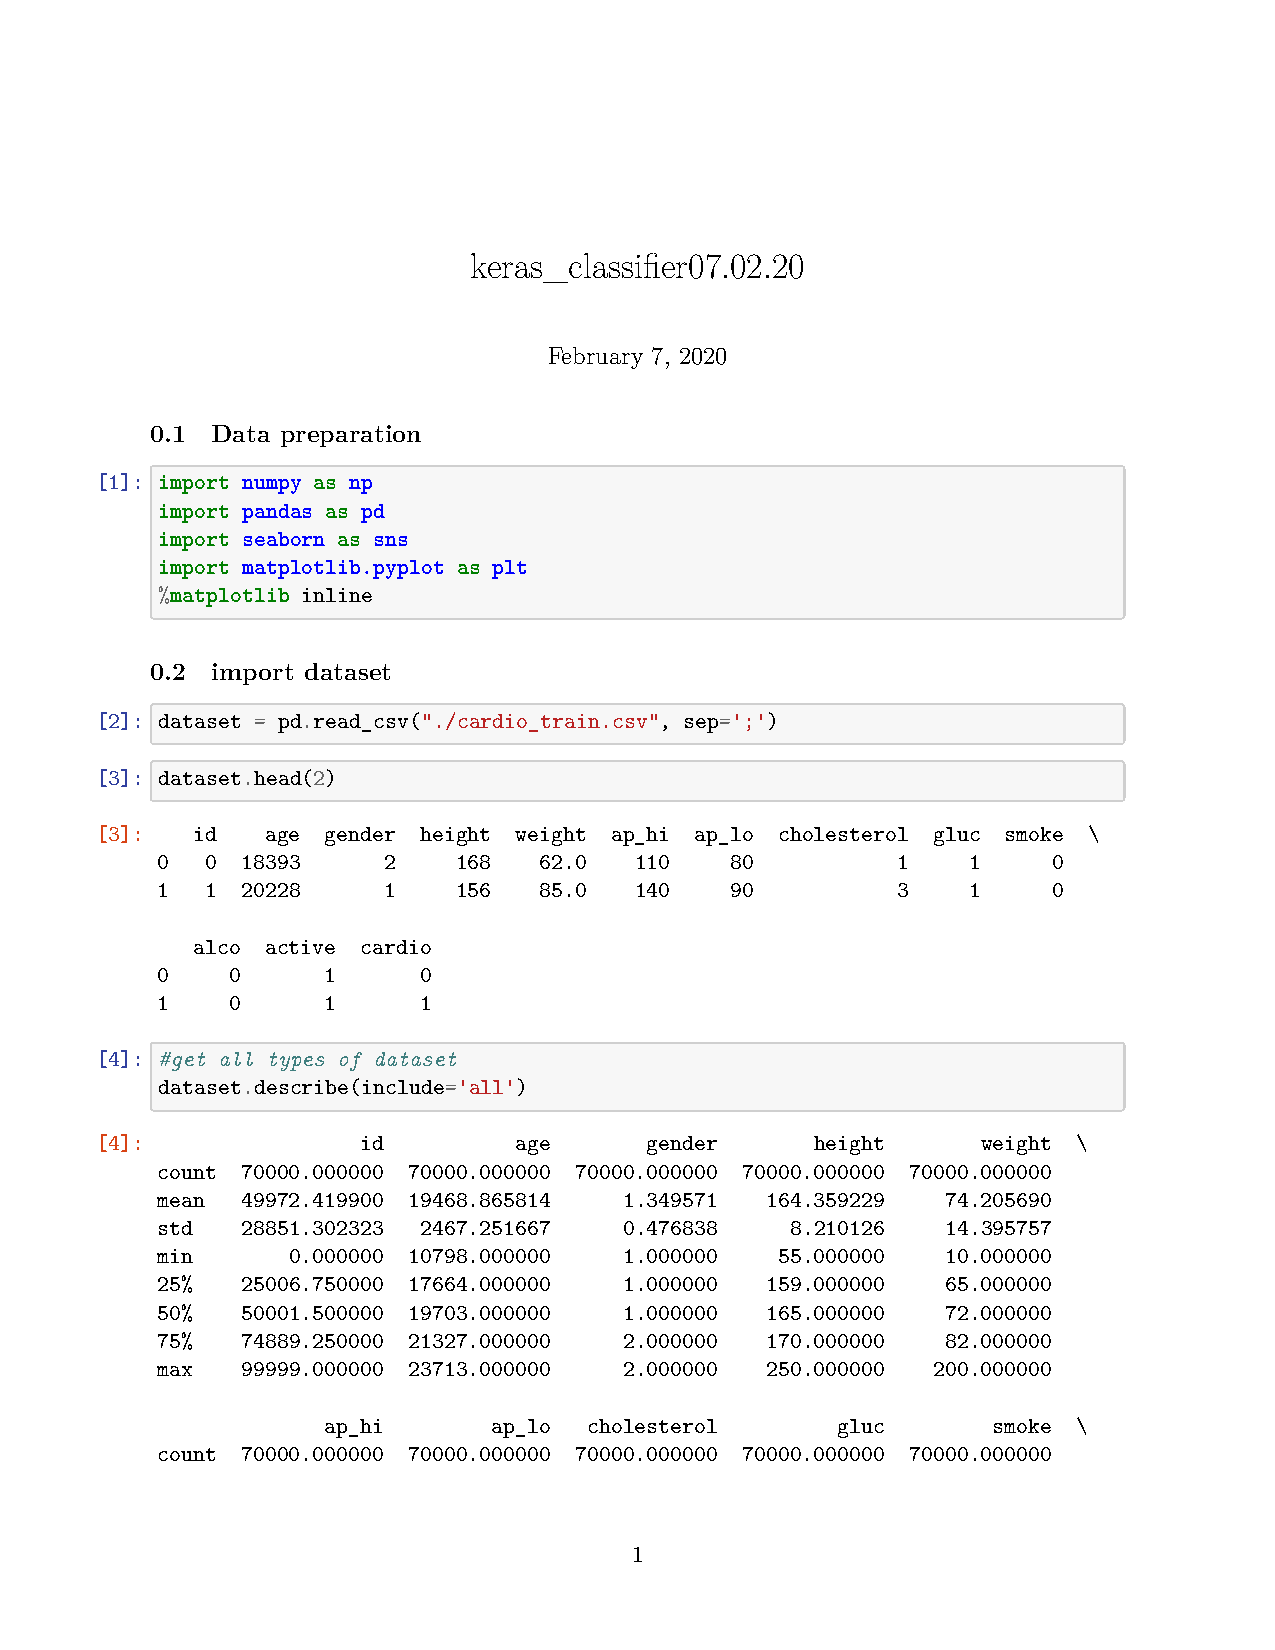
\includepdf[pages=-]{keras_classifier.pdf}

\end{document}
